\documentclass{book}

\usepackage{fontspec} % used to import Calibri
\usepackage{anyfontsize} % used to adjust font size

% needed for inch and other length measurements
% to be recognized
\usepackage{calc}

% for colors and text effects as is hopefully obvious
\usepackage[dvipsnames]{xcolor}
\usepackage{soul}

% control over margins
\usepackage[margin=1in]{geometry}
\usepackage[strict]{changepage}

\usepackage{mathtools}
\usepackage{amsfonts}
\usepackage{bm}

\usepackage[scr=rsfso, scrscaled=.96]{mathalpha}

% This is how I'm getting the nice caligraphy font :(
\DeclareMathAlphabet{\eulerscr}{U}{eus}{m}{n}
\newcommand{\mathcalli}[1]{\text{\scalebox{1.11}{$\eulerscr{#1}$}}}


\usepackage{amssymb} % originally imported to get the proof square
\usepackage{xfrac}
\usepackage[overcommands]{overarrows} % Get my preferred vector arrows...
\usepackage{relsize}

% Just am using this to get a dashed line in a table...
% Also you apparently want this to be inactive if you aren't
% using it because it slows compilation.
\usepackage{arydshln} \ADLinactivate 
\newenvironment{allowTableDashes}{\ADLactivate}{\ADLinactivate}

\usepackage{graphicx}
\graphicspath{{./158_Images/}}

\usepackage{tikz}
   \usetikzlibrary{arrows.meta}
   \usetikzlibrary{graphs, graphs.standard}

\usepackage{quiver} %commutative diagrams






\usepackage[hidelinks]{hyperref}
\newcommand{\inLinkRap}[2]{{\color{blue}\hyperlink{#1}{\textit{#2}}}}







\newfontfamily{\calibri}{Calibri}
\setlength{\parindent}{0pt}
\definecolor{RawerSienna}{HTML}{945D27}

% ~~~~~~~~~~~~~~~~~~~~~~~~~~~~~~~~~~~~~~~~~~~~~~~~~~
%Arrow Commands:

% Thank you Bernard, gernot, and Sigur who I copied this from:
% https://tex.stackexchange.com/questions/364096/command-for-longhookrightarrow
\renewcommand{\hookrightarrow}{\lhook\joinrel\rightarrow}
\renewcommand{\hookleftarrow}{\leftarrow\joinrel\rhook}
\newcommand{\hooklongrightarrow}{\lhook\joinrel\longrightarrow}
\newcommand{\hooklongleftarrow}{\longleftarrow\joinrel\rhook}
\newcommand{\hookxlongrightarrow}[2][]{\lhook\joinrel\xrightarrow[#1]{#2}}
\newcommand{\hookxlongleftarrow}[2][]{\xleftarrow[#1]{#2}\joinrel\rhook}

% Thank you egreg who I copied from:
% https://tex.stackexchange.com/questions/260554/two-headed-version-of-xrightarrow
\newcommand{\longrightarrowdbl}{\longrightarrow\mathrel{\mkern-14mu}\rightarrow}
\newcommand{\longleftarrowdbl}{\leftarrow\mathrel{\mkern-14mu}\longleftarrow}

\newcommand{\xrightarrowdbl}[2][]{%
  \xrightarrow[#1]{#2}\mathrel{\mkern-14mu}\rightarrow
}
\newcommand{\xleftarrowdbl}[2][]{%
  \leftarrow\mathrel{\mkern-14mu}\xleftarrow[#1]{#2}
}

\newcommand{\mRoman}[1]{%
   \textrm{\MakeUppercase{\romannumeral #1}}%
}



% ~~~~~~~~~~~~~~~~~~~~~~~~~~~~~~~~~~~~~~~~~~~~~~~~~~

\newcommand{\hOne}{%
   \color{Black}%
   \fontsize{14}{16}\selectfont%
}
\newcommand{\hTwo}{%
\color{Black}%
   \fontsize{13}{15}\selectfont%
}
% \newcommand{\scratchWork}{%
%    \color{PineGreen!85!Orange}
%    \fontsize{12}{14}\selectfont%
% }
\newcommand{\hThree}{%
   \color{Black}%
   \fontsize{12}{14}\selectfont%
}
\newcommand{\myComment}{%
   \color{RawerSienna}%
   \fontsize{12}{14}\selectfont%
}
\newcommand{\pracOne}{
   \color{BrickRed}%
   \fontsize{13}{15}\selectfont%
}
\newcommand{\pracTwo}{
   \color{Orange}%
   \fontsize{12}{14}\selectfont%
}
\newcommand{\why}{%
   \color{Orange}%
   \fontsize{12}{14}\selectfont%
	Why:
}
\newcommand{\exOne}{%
   \color{Purple}%
   \fontsize{14}{16}\selectfont%
}
\newcommand{\exTwo}{%
   \color{Purple}%
   \fontsize{13}{15}\selectfont%
}
\newcommand{\exThree}{%
   \color{Purple}%
   \fontsize{12}{14}\selectfont%
}
\newcommand{\exP}{%
   \color{Purple}%
   \fontsize{12}{14}\selectfont%
}
\newcommand{\exTwoP}{%
   \color{RedViolet}%
   \fontsize{13}{15}\selectfont%
}
\newcommand{\exThreeP}{%
   \color{RedViolet}%
   \fontsize{12}{14}\selectfont%
}
\newcommand{\exFourP}{%
   \color{RedViolet}%
   \fontsize{11}{13}\selectfont%
}
\newcommand{\exPP}{%
   \color{RedViolet}%
   \fontsize{12}{14}\selectfont%
}
\newcommand{\exPPP}{%
   \color{VioletRed}%
   \fontsize{12}{14}\selectfont%
}

% Homework standard below (God the bloat in the header is absurd...)
% ~~~~~~~~~~~~~~~~~~~~~~~~~~~~~~~~~~~~~~~~~~~~~~~~
\newcommand{\Hstatement}{%
   \color{MidnightBlue!90!Black}%
   \fontsize{12}{13}\selectfont%
}
\newcommand{\HexOne}{%
   \color{Purple}%
   \fontsize{12}{13}\selectfont%
}
\newcommand{\HexTwoP}{%
   \color{RedViolet}%
   \fontsize{12}{13}\selectfont%
}
\newcommand{\HexPPP}{%
   \color{VioletRed}%
   \fontsize{11}{12}\selectfont%
}

% ~~~~~~~~~~~~~~~~~~~~~~~~~~~~~~~~~~~~~~~~~~~~~~~~

\newcommand{\cyPen}[1]{{\vphantom{.}\color{Cerulean}#1}}
\newcommand{\redPen}[1]{{\vphantom{.}\color{Red}#1}}

\newenvironment{myIndent}{%
   \begin{adjustwidth}{2.5em}{0em}%
}{%
   \end{adjustwidth}%
}

\newenvironment{myDindent}{%
   \begin{adjustwidth}{5em}{0em}%
}{%
   \end{adjustwidth}%
}

\newenvironment{myTindent}{%
   \begin{adjustwidth}{7.5em}{0em}%
}{%
   \end{adjustwidth}%
}

\newenvironment{myConstrict}{%
   \begin{adjustwidth}{2.5em}{2.5em}%
}{%
   \end{adjustwidth}%
}

\newcommand{\udefine}[1]{{%
   \setulcolor{Red}%
   \setul{0.14em}{0.07em}%
   \ul{#1}%
}}

\newcommand{\uprop}[1]{{%
   \setulcolor{Purple}%
   \setul{0.14em}{0.07em}%
   \ul{#1} 
}}

\newcommand{\blab}[1]{\textbf{#1}}
\newcommand{\blect}[1]{{\color{MidnightBlue}\textbf{#1}}}

\newcommand{\uuline}[2][.]{%
{\vphantom{a}\color{#1}%
\rlap{\rule[-0.18em]{\widthof{#2}}{0.06em}}%
\rlap{\rule[-0.32em]{\widthof{#2}}{0.06em}}}%
#2}

\newcommand{\pprime}{{\prime\prime}}
\newcommand{\suchthat}{ \hspace{0.3em}s.t.\hspace{0.3em}}
\newcommand{\rea}[1]{\mathrm{Re}(#1)}
\newcommand{\ima}[1]{\mathrm{Im}(#1)}
\newcommand{\comp}{\mathsf{C}}
\newcommand{\trans}{\mathsf{T}}
\newcommand{\myHS}{ \hspace{0.5em}}
\newcommand{\gap}{\phantom{2}}

\newcommand{\GenLin}{\ensuremath{\mathrm{GL}}}
\newcommand{\Cay}{\ensuremath{\mathrm{Cay}}}

\newcommand{\myId}{\mathrm{Id}}
\newcommand{\myIm}{\mathrm{im}}
\newcommand{\Obj}{\mathrm{Obj}}
\newcommand{\Hom}{\mathrm{Hom}}
\newcommand{\End}{\mathrm{End}}
\newcommand{\Aut}{\mathrm{Aut}}

\newcommand{\df}{\mathrm{d}}
\newcommand{\Df}{\mathrm{D}}

\newcommand{\mcateg}[1]{{\bm{\mathsf{#1}}}}

\newcommand{\mdeg}{\mathrm{mdeg}\phantom{.}}

\newcommand{\divides}{\mathop{\mid}}

\newcommand{\card}{\mathrm{card}}
\newcommand{\supp}{\mathrm{supp}}
\newcommand{\diam}{\mathrm{diam}}
\newcommand{\conv}{\mathrm{conv}}
\newcommand{\opnorm}{\mathrm{op}}
\newcommand{\loc}{\mathrm{loc}}
\newcommand{\sgn}{\mathrm{sgn}}
\newcommand{\acc}{\mathrm{acc}}

\newcommand{\mSpan}{\mathrm{span}}
\newcommand{\Interior}{\mathop{\mathrm{Int}}}

\newcommand{\mMat}[1]{\mathbf{#1}}

\newcommand{\NBV}{\ensuremath{\mathrm{NBV}}}
\newcommand{\Acc}{\mathrm{Acc}}
\newcommand{\BV}{\ensuremath{\mathrm{BV}}}
\newcommand{\Var}{\ensuremath{\mathrm{Var}}}

\newcommand{\Alt}{\mathrm{Alt}}
\newcommand{\Sym}{\mathrm{Sym}}

\newcommand{\weakst}{weak$^*$ }

\newcommand{\radtimes}{\mathop{\widehat{\times}}}

\newcommand{\mMod}[1]{\phantom{a}(\mathrel{\mathrm{mod}} #1)}
\newcommand{\Fun}{\mathrm{Fun}}
\newcommand{\act}{\mathrm{act}}
\newcommand{\Fix}{\mathrm{Fix}}
\newcommand{\Sub}{\mathrm{Sub}}
\newcommand{\Cl}{\mathrm{Cl}}
\newcommand{\GL}{\mathrm{GL}}
\newcommand{\SL}{\mathrm{SL}}
\newcommand{\core}{\mathrm{core}}
\newcommand{\Syl}{\mathrm{Syl}}
\newcommand{\Iso}{\mathrm{Iso}}
\newcommand{\Homeo}{\mathrm{Homeo}}
\newcommand{\Inn}{\mathrm{Inn}}


\DeclareMathOperator{\lcm}{lcm}
\DeclareMathOperator{\symdif}{\triangle}
\DeclareMathOperator{\Average}{Average}
\DeclareMathOperator*{\AverageAst}{Average}

% Thank you Gonzalo Medina and Moriambar who wrote this on stack exchange:
%https://tex.stackexchange.com/questions/74125/how-do-i-put-text-over-symbols%
\newcommand{\myequiv}[1]{\stackrel{\mathclap{\mbox{\footnotesize{$#1$}}}}{\equiv}}

% Thank you chs who wrote this on stack exchange:
%https://tex.stackexchange.com/questions/89821/how-to-draw-a-solid-colored-circle%
\newcommand{\filledcirc}[1][.]{\ensuremath{\hspace{0.05em}{\color{#1}\bullet}\mathllap{\circ}\hspace{0.05em}}}

%Thank you blerbl who wrote this on stack exchange:
%https://tex.stackexchange.com/questions/25348/latex-symbol-for-does-not-divide
\newcommand{\ndiv}{\hspace{-0.3em}\not|\hspace{0.35em}}

\newcommand{\mySepOne}[1][.]{%
   {\noindent\color{#1}{\rule{6.5in}{1mm}}}\\%
}
\newcommand{\mySepTwo}[1][.]{%
   {\noindent\color{#1}{\rule{6.5in}{0.5mm}}}\\%
}
\newcommand{\mySepThree}[1][.]{%
   {\noindent\color{#1}{\rule{6in}{0.25mm}}}\\%
}

\newenvironment{myClosureOne}[2][.]{%
   \color{#1}%
   \begin{tabular}{|p{#2in}|} \hline \\%
}{%
   \\ \hline \end{tabular}%
}

\newcommand{\retTwo}{\hfill\bigbreak}

\newcommand{\dispDate}[1]{{
   \color{Black}%
   \fontsize{20}{18}\selectfont%
   #1\retTwo
}}


\begin{document}
\setul{0.14em}{0.07em}
\calibri

\hTwo \hypertarget{math 200a lecture 6}{\blect{Math 200a (lecture 6)}}\retTwo

\exTwo\ul{Sylow's 2nd. Theorem:} Suppose $P_0 \in \Syl_p(G)$ and $Q$ is a $p$-subgroup of $G$. Then there exists $x \in G$ such that $Q \subseteq xP_0 x^{-1}$.

\begin{myIndent}\exThreeP
	Proof:\\
	$Q \curvearrowright G / P_0$ by left-translation. Then by the theorem in the middle of \inLinkRap{Alireza theorem page 271}{page 271}, we\\ have that $|G / P_0| \equiv |(G/P_0)^Q| \mMod{p}$. But since $P_0 \in \Syl_p(G)$, we have that\\ $|G/P_0| \not\equiv 0 \mMod{p}$. Hence, there must exist some $gP_0 \in (G / P_0)^Q$.\retTwo

	In turn, $xgP = gP$ for all $x \in Q$. Or in other words, $g \in gPg^{-1}$ for all $x \in Q$. Hence, $Q \subseteq gPg^{-1}$. $\blacksquare$\retTwo
\end{myIndent}

\ul{Corollary:} If $P_1, P_2 \in \Syl_p(G)$ then there exists $g \in G$ such that $gP_1g^{-1} = P_2$.

\begin{myIndent}\exThreeP
	Proof:\\
	By Sylow's 2nd theorem we know there exists $g \in G$ such that $P_2 \subseteq gP_1g^{-1}$. And since $|P_2| = |P_1|$ we deduce $P_2 = gP_1g^{-1}$. $\blacksquare$\retTwo
\end{myIndent}

\hTwo Note the following observations:\\ [-20pt]
\begin{itemize}
	\item If $\theta \in \Aut(G)$ and $P \in \Syl_p(G)$ then $\theta(P) \in \Syl_p(G)$.
	\item $G \curvearrowright \Syl_p(G)$ by conjugation and this actions is transitive (by the last corollary).
	\item A subgroup $H < G$ is called a \udefine{characteristic} subgroup if $\forall \theta \in \Aut(G)$ we have\\ that $\theta(H) = H$. By the last two observations, if $\Syl_p(G) = \{P\}$, then $P$ is a\\ characteristic subgroup of $G$ {\color{BrickRed}(which automatically means $P$ is normal since\\ conjugation is an automorphism of $G$)}.\retTwo
\end{itemize}

\exTwo\ul{Corollary:} If $P \lhd G$ and $P \in \Syl_p(G)$, then $P$ is a characteristic subgroup of $G$.

\begin{myIndent}\exThreeP
	Proof:\\
	Since $P \lhd G$, $P \in \Syl_p(G)$, and $G \curvearrowright \Syl_p(G)$ transitively via conjugation, we must have that $\Syl_p(G) = \{P\}$. Hence $P$ is a characteristic subgroup of $G$. $\blacksquare$\retTwo
\end{myIndent}

\hTwo\mySepTwo

\exTwo\ul{Lemma:} If $P \in \Syl_p(G)$, then $\Syl_p(N_G(P)) = \{P\}$.

\begin{myIndent}\exThreeP
	Proof:\\
	We know $|P| = p^{\nu_p(|G|)}$. Also, $P < N_G(P) < G$ means that $|P|$ divides $|N_G(P)|$ and $|N_G(P)|$ divides $|G|$. Thus $\nu_p(|G|) = \nu_p(|N_G(P)|)$ and so $P \in \Syl_p(N_G(P))$. Finally, since $P \lhd N_G(P)$, we know from the last corollary that $\Syl_p(N_G(P)) = \{P\}$. $\blacksquare$\retTwo
\end{myIndent}

\ul{Lemma:} If $P_0 \in \Syl_p(G)$ and we consider $P_0 \curvearrowright \Syl_p(G)$ by conjugation, then\\ $(\Syl_p(G))^{P_0} = \{P_0\}$.

\begin{myIndent}\exThreeP
	Proof:\\
	$P \in (\Syl_p(G))^{P_0}$ if and only if for all $x\in P_0$, $xPx^{-1} = P$. That's to say, iff $P_0 \subseteq N_G(P)$. But that would mean $P_0 \in \Syl_p(N_G(P)) = \{P\}$. So $(\Syl_p(G))^{P_0} = \{P_0\}$. $\blacksquare$\newpage
\end{myIndent}

\ul{Sylow's 3rd. Theorem:} If $G$ is a finite group, $|\Syl_p(G)| \equiv 1 \mMod{p}$.

\begin{myIndent}\exThreeP
	Proof:\\
	Suppose $P_0 \in \Syl_p(G)$. Then $|\Syl_p(G) \equiv |(\Syl_p(G))^{P_0} \mMod{p}$. But from the prior lemma we know $|(\Syl_p(G))^{P_0}| = 1$. $\blacksquare$\retTwo

	\myComment So as a recap, suppose $G$ is a finite group and $p$ is a prime number dividing $|G|$. Then:
	\begin{itemize}
		\item Sylow's first theorem guarentees that $\Syl_p(G) \neq \emptyset$.
		\item Sylow's third theorem guarentees that $|\Syl_p(G)| \equiv 1 \mMod{p}$.
		\item Sylow's second theorem guarentees that $|\Syl_p(G)|$ equals the number of conjugates of $P_0$ where $P_0 \in \Syl_p(G)$. Thus (see  \inLinkRap{page 271 reference}{page 271}), we have for any $P_0 \in \Syl_p(G)$ that $|\Syl_p(G)| = [G : N_G(P_0)]$. And in particular, since $P_0 < N_G(P_0) < G$, we have that $|\Syl_p(G)| = \frac{|G|}{|N_G(P_0)|} = \frac{[G : P_0]|P_0|}{[N_G(P_0) : P_0]|P_0|} = \frac{[G : P_0]}{[N_G(P_0) : P_0]}$. So $|\Syl_p(G)|$ divides $[G : P_0]$.\retTwo
	\end{itemize}
\end{myIndent}

\ul{Proposition:} $P \in \Syl_p(G) \Longrightarrow N_G(N_G(P)) = N_G(P)$.

\begin{myIndent}\exThreeP
	Proof:\\
	The $\supseteq$ inclusion is obvious. Meanwhile, $x \in N_G(N_G(P))$ implies that\\ $xN_G(P)x^{-1} = N_G(P)$. But note that if $\theta \in \Aut(G)$ and $H < G$, then\\ $\theta(N_G(H)) = N_G(\theta(H))$.

	\begin{myIndent}\exPPP
		If $x \in N_G(H)$ then we know that $xHx^{-1} = H$. So:
		
		{\centering $\phi(x)\phi(H)\phi(x)^{-1} = \phi(xHx^{-1}) = \phi(H)$.\retTwo\par}
		
		This shows that $\phi(x) \in N_G(\phi(H))$ and hence $\phi(N_G(H)) \subseteq N_G(\phi(H))$ whenever $\phi \in \Aut(G)$. Using this fact, now note that for any $\phi \in \Aut(G)$, we have that:
		
		{\centering$N_G(H) = \phi^{-1}(\phi(N_G(H))) \subseteq \phi^{-1}(N_G(\phi(H))) \subseteq N_G(\phi^{-1}(\phi(H))) = N_G(H)$\retTwo\par}

		So, $N_G(H) = \phi^{-1}(N_G(\phi(H)))$. And by composing $\phi$ we get that:
		
		{\centering$\phi(N_G(H)) = N_G(\phi(H))$.\retTwo\par}
	\end{myIndent}

	It follows that $N_G(xPx^{-1}) = xN_G(P)x^{-1} = N_G(P)$ whenever $x \in N_G(N_G(P))$. But in that case we have that $\Syl_p(N_G(xPx^{-1})) = \Syl_p(N_G(P))$. And as $P$ and $xPx^{-1}$ are both Sylow $p$-groups, we conclude $xPx^{-1} = P$. So $x \in N_G(P)$
\end{myIndent}

\hTwo\mySepTwo

I probably should have been taught this in math 100a but never was. So, I guess I'll just refresh myself now. The book I'm following along with is \textit{Abstract Algebra} by Dummit and Foote.\retTwo

Suppose $G$ is a group and $H, K$ are subgroups of $G$. Then we define:

{\centering$HK \coloneqq \{ hk \in G : h \in H \text{ and } k \in K\}$.\retTwo\par}

\exTwo\ul{Proposition 3.2.13:} If $H$ and $K$ are finite subgroups of a group, then $|HK| = \frac{|H||K|}{|H\cap K|}$.

\begin{myIndent}\exThreeP
	Proof:\\
	Note that $HK = \bigcup_{h \in H} hK$. Thus $|HK|$ equals $|K|$ times the number of distinct left cosets $hK$ where $h \in H$. But note that for any $h_1, h_2 \in H$:
	
	{\centering$h_1 K = h_2 K \Longleftrightarrow h_2^{-1}h_1 \in H \cap K \Longleftrightarrow h_1 (H \cap K) = h_2 (H \cap K)$.\newpage\par}

	Hence $|HK| = |K| \cdot [H : H \cap K] = |K|\frac{|H|}{|H \cap K|}$ by Lagrange's theorem. $\blacksquare$\retTwo
\end{myIndent}

\ul{Proposition 3.2.14:} If $H$ and $K$ are subgroups of $G$, then $HK < G$ iff $HK = KH$.

\begin{myIndent}\exThreeP
	$(\Longrightarrow)$\\
	Suppose $HK < G$. Since $K < HK$ and $H < HK$, we thus know that $KH \subseteq HK$.\\ Meanwhile, suppose $h \in H$ and $k \in K$. Since $HK$ is a group, we know $(hk)^{-1} \in HK$.\\ So there exists $h^\prime \in H$ and $k^\prime \in K$ such that $(hk)^{-1} = h^\prime k^\prime$. But then $hk = (k^\prime)^{-1}(h^\prime)^{-1}$\\ which is in $KH$. So $HK \subseteq KH$.\retTwo

	$(\Longleftarrow)$\\
	Assume $HK = KH$ and let $a, b \in HK$. Then there exists $h_1, h_2 \in H$ and $k_1, k_2 \in K$ such that $a = h_1k_1$ and $b = h_2k_2$. Now it's clear that $1_G \in HK$. So, if we can show that $ab^{-1} \in HK$, then we will know that $HK$ is a group.\retTwo
	
	Fortunately, $ab^{-1} = h_1k_1k_2^{-1}h_2^{-1}$. And since $KH = HK$, we know there is $h_3 \in H$ and $k_3 \in K$ such that $(k_1k_2^{-1})h_2^{-1} = h_3 k_3$. Thus, $ab^{-1} = (h_1h_3)(k_3) \in HK$. $\blacksquare$\retTwo
\end{myIndent}

\ul{Corollary 3.2.15:} If $H$ and $K$ are subgroups of $G$ and $H < N_G(K)$, then $HK$ is a subgroup of $G$. In particular, if $K \lhd G$ then $HK < G$ for any $H < G$.

\begin{myIndent}\exThreeP
	Proof:\\
	Let $h \in H$ and $k \in K$. Then $hkh^{-1} \in K$. So $hk = (hkh^{-1})h \in KH$ and we've proven that $HK = KH$. $\blacksquare$\retTwo
\end{myIndent}

\ul{Second Isomorphism Theorem:} Let $G$ be a group, let $A$ and $B$ be subgroups of $G$, and assume $A < N_G(B)$. Then $AB < G$, $B \lhd AB$, $A \cap B \lhd A$, and $AB/B \cong A/(A\cap B)$.

\begin{myIndent}\exThreeP
	Proof:\\
	By the last corollary we know that $AB < G$. Also, since $A < N_G(B)$ and $B < N_G(B)$, it follows $AB < N_G(B)$. Hence $B \lhd AB$.\retTwo

	Now we know there is a well-defined group homomorphism $\phi: A \to AB/B$ given by $\phi(a) = aB$. Clearly $\phi$ is surjective. Meanwhile, it's easy to see that $\ker(\phi) = A \cap B$. So by the first isomorphism theorem, we have that $A \cap B \lhd A$ and that:
	
	{\centering $AB/B \cong A/(A\cap B)$. $\blacksquare$\retTwo\par}
\end{myIndent}

\hTwo Here is one more miscellaneous result before getting back to the lecture:\retTwo

\exTwo\ul{Lemma:} If $N_1, N_2 \lhd G$, then $\forall x \in N_1$ and $\forall y \in N_2$ we have that $xyx^{-1}y^{-1} \in N_1 \cap N_2$.

\begin{myIndent}\exThreeP
	Proof:\\
	$(xyx^{-1}) \in N_2$ and $(yx^{-1}y^{-1}) \in N_1$ since both $N_1$ and $N_2$ are normal. Hence:
	
	{\centering$(xyx^{-1})y^{-1} = x(yx^{-1}y^{-1}) \in N_1 \cap N_2$. $\blacksquare$\retTwo\par}
\end{myIndent}

\ul{Corollary:} If $N_1, N_2 \lhd G$ and $N_1 \cap N_2 = \{1\}$, then $xy = yx$ for all $x \in N_1$ and $y \in N_2$.

\hTwo\mySepTwo

So here are some uses of Sylow's theorems:
\begin{itemize}
	\item Suppose $p < q$ are distinct primes with $p \not\divides q- 1$. If $|G| = pq$ then $G \cong C_{pq}$.
	
	\begin{myIndent}\pracTwo
		Let $s_q$ and $s_p$ be shorthand for $|\Syl_q(G)|$ and $|\Syl_p(G)|$. Now we know by Sylow's third theorem that $s_q \equiv 1 \mMod{q}$.\newpage
		
		Also, we know that $s_q \divides p$ by Sylow's second theorem. And since $p < q$, we must have that $s_q = 1$. Hence $\Syl_q(G) = \{Q\}$ for some $Q \lhd G$ such that $|Q| = q$ and $Q$ is cylic of order $q$.\retTwo

		Next, note once again by Sylow's second theorem that $s_p \divides q$. Hence, we must have that either $s_p = 1$ or $s_p = q$. That said, we know $q - 1 \not\equiv 0 \mMod{p}$ by assumption and that $s_p \equiv 1 \mMod{p}$ by Sylow's third theorem. So, we must have that $s_p = 1$ and it follows that $\Syl_p(G) = \{P\}$ for some $P \lhd G$ such that $|P| = p$ and $P$ is cyclic of order $p$.\retTwo

		Now $|P \cap Q| \divides \gcd(|P|, |Q|) = 1$. So $P \cap Q = \{1\}$. And by our prior corollary, this means that $xy = yx$ for all $x \in P$ and $y \in Q$.\retTwo

		Now consider the map $f : P \times Q \to G$ given by $(x, y) \mapsto xy$. We claim this is a group isomorphism.
		\begin{itemize}
			\item[$\bullet$] Note that:
			
			{\centering\begin{tabular}{l}
				$f(x_1, y_1)f(x_2, y_2) = x_1y_1x_2y_2 = x_1x_2y_1y_2$\\
				$\phantom{f(x_1, y_1)f(x_2, y_2) = x_1y_1x_2y_2} = f(x_1x_2, y_1y_2) = f((x_1, y_1)(x_2,y_2))$.
			\end{tabular}\retTwo\par}

			Thus $f$ is a group homomorphism.\retTwo

			\item[$\bullet$] Suppose $f(x, y) = 1$. Then $xy = 1$ which means that $x = y^{-1}$. But now $x, y^{-1} \in P \cap Q = \{1\}$. So $(x, y) = (1, 1)$ and we've shown that $f$ is injective.\retTwo
			
			\item[$\bullet$] $|\myIm(f)| = |PQ| = \frac{|P||Q|}{|P \cap Q|} = \frac{pq}{1} = |G|$. So $f$ is surjective.\retTwo
		\end{itemize}

		It follows that $G \cong P \times Q \cong \mathbb{Z}/p\mathbb{Z} \times \mathbb{Z}/q\mathbb{Z} \cong \mathbb{Z}/pq\mathbb{Z}$. (The last equivalence is from Chinese remainder theorem\dots)
	\end{myIndent}
\end{itemize}

I am not fully caught up with this class yet. But, I'll stop here for now so that I can go back to taking functional analysis notes. For more math 200a notes go to \inLinkRap{math 200a lecture 7}{page \_\_\_}.

\mySepTwo

\dispDate{10/14/2025}

\hypertarget{more function analysis lectures 3-5}{\blect{Math 241a (lectures 3-5 continued):}}\retTwo

If $\mathcalli{X}$ is a topological vector space, then here is one more topology on $\mathcalli{X}^*$ to be aware of.

\begin{myIndent}\hThree
	Let $\mathcalli{A}$ be the collection of all (Von-Neumann) bounded sets in $\mathcalli{X}$ and then for each $A \in \mathcalli{A}$ define the seminorm $p_A(\lambda) = \sup_{x \in A} |\lambda(x)|$ on $\mathcalli{X}^*$. Since every singleton is bounded, we know this defines a sufficient family. Also, the topology generated by that family is finer than the \weakst topology. So, we call it the \udefine{strong topology} on $\mathcalli{X}^*$.\retTwo
\end{myIndent}

(\ul{Definition 1.2.19:}) If $\mathcalli{X}$, $\mathcalli{Y}$ are topological ($K$-)vector spaces and $T \in B(\mathcalli{X}, \mathcalli{Y})$, then $T$'s \udefine{adjoint} is defined as the map $T^* : \mathcalli{Y}^* \to \mathcalli{X}^*$ given by $T^*(\lambda) = \lambda \circ T$.\newpage

Note that:
\begin{itemize}
	\item $T^*$ is a well-defined linear operator.
	
	\begin{myIndent}\pracTwo
		To show that $T^*$ is well defined, suppose $c_1, c_2 \in K$ and $x_1, x_2 \in \mathcalli{X}$. Then:

		{\centering\begin{tabular}{l}
			$T^*(\lambda)(c_1x_1 + c_2x_2) = \lambda(T(c_1x_1 + c_2x_2))$\\ [4pt]
			$\phantom{T^*(\lambda)(c_1x_1 + c_2x_2)} = c_1\lambda(T(x_1)) + c_2\lambda(T(x_2)) = c_1T^*(\lambda)(x_1) + c_2T^*(\lambda)(x_2)$. 
		\end{tabular}\retTwo\par}

		Next, to show that $T^*$ is linear, suppose $c_1, c_2 \in K$ and $\lambda_1, \lambda_2 \in \mathcalli{Y}^*$. Then for any $x \in \mathcalli{X}$ we have that:

		{\centering\begin{tabular}{l}
			$T^*(c_1\lambda_1 + c_2\lambda_2)(x) = (c_1\lambda_1 + c_2\lambda_2)(T(x))$\\ [4pt]
			$\phantom{T^*(c_1\lambda_1 + c_2\lambda_2)(x)} = c_1\lambda_1(T(x)) + c_2\lambda_2(T(x)) = c_1T^*(\lambda_1)(x) + c_2T^*(\lambda_2)(x)$\\ [4pt]
			$\phantom{T^*(c_1\lambda_1 + c_2\lambda_2)(x) = c_1\lambda_1(T(x)) + c_2\lambda_2(T(x))} = (c_1T^*(\lambda_1) + c_2T^*(\lambda_2))(x)$\\ [4pt]
		\end{tabular}\par}
	\end{myIndent}

	\item $T^*$ is continuous if $\mathcalli{X}^*$ and $\mathcalli{Y}^*$ are equipped with the \weakst topologies.
	
	\begin{myIndent}\pracTwo
		This is because if $\lambda_{\beta}(y) \to \lambda(y)$ for all $y \in \mathcalli{Y}$ then $\lambda_{\beta}(Tx) \to \lambda(\beta)(Tx)$ for all $x \in \mathcalli{X}$. Hence, we have for any \weakst\hspace{-0.4em}-ly convergent net $\langle \lambda_{\beta}\rangle$ that $\langle T^*(\lambda_\beta)\rangle$ is also \weakst\hspace{-0.4em}-ly convergent.
	\end{myIndent}

	\item $T^*$ is also continuous if $\mathcalli{X}^*$ and $\mathcalli{Y}^*$ are equipped with the strong topologies.

	\begin{myIndent}\pracTwo
		This is because if $T$ is continuous, then $T$ maps bounded sets to bounded sets.
		\begin{myIndent}
			Proof:\\
			Suppose $A \subseteq \mathcalli{X}$ is bounded and let $N$ be any neighborhood of $0 \in \mathcalli{Y}$. Because $T$ is continuous, we know that $T^{-1}(N)$ is a neighborhood of $0 \in \mathcalli{X}$. And since $A$ is bounded, there is some $r > 0$ such that $A \subseteq sT^{-1}(N)$ for all $s \in K$ with $|s| \geq r$. In turn, $T(A) \subseteq T(sT^{-1}(N)) = sT(T6{-1}(N)) = sN$ whenever $|s| \geq r$. And this proves that $T(A) \subseteq \mathcalli{Y}$ is bounded.\retTwo
		\end{myIndent}

		Thus by similar logic to the last bullet point, if $\langle \lambda_{\beta}\rangle$ is a strongly convergent net then $\langle T^*(\lambda_\beta)\rangle$ is also a strongly convergent net.\retTwo

		\begin{myIndent}\myComment
			As a side note, technically only the third bullet point actually required the\\ continuity of $T$.\retTwo
		\end{myIndent}
	\end{myIndent}
\end{itemize}

\exTwo\ul{Lemma 1.2.21:} If $\mathcalli{X}$ and $\mathcalli{Y}$ are normed vector spaces and $T \in B(\mathcalli{X}, \mathcalli{Y})$, then\\ $\|T^*\|_{\opnorm} = \|T\|_{\opnorm}$.

\begin{myIndent}\exThreeP
	Proof:\\
	For all $x \in \mathcalli{X}$ and $\lambda \in \mathcalli{Y}^*$, we have that $|T^*(\lambda)(x)| = |\lambda(Tx)| \leq \|\lambda\|\|T\|\|x\|$.\\ So $\|T^*(\lambda)\| \leq \|\lambda\|\|T\|$ for all $\lambda \in \mathcalli{Y}^*$. And this shows that $\|T^*\| \leq \|T\|$.\retTwo

	On the other hand, for all $\varepsilon > 0$ there exists $x \in E$ such that $\|x\|=1$ and\\ $\|Tx\| \geq \|T\| - \varepsilon$. Also, as a consequence of the Hahn Banach theorem (see\\ Folland theorem 5.8 in my math 240b notes), there exists $\lambda \in \mathcalli{Y}^*$ such that\\ $\lambda(Tx) = \|Tx\|$ and $\|\lambda\| = 1$. So:

	{\center\begin{tabular}{l}
		$\|T^*\| \geq \|\lambda\|^{-1}\|T^*(\lambda)\|$\\ [2pt]
		$\phantom{\|T^*\|} = 1 \cdot \|T^*(\lambda)\| \geq \|x\|^{-1} |T^*(\lambda)(x)|$\\ [2pt]
		$\phantom{\|T^*\| = 1 \cdot \|T^*(\lambda)\|} = 1 \cdot |T^*(\lambda)(x)| = |\lambda(Tx)| = \|Tx\| \geq \|T\| - \varepsilon$. $\blacksquare$
	\end{tabular}\newpage\par}
\end{myIndent}

\hTwo Let $\mathcalli{H}$ be a real of complex Hilbert space. Then recall that there is an isometric bijection  $i : \mathcalli{H} \to \mathcalli{H}^*$ where we identify every $x \in \mathcalli{H}$ with the linear functional $i(x) \coloneqq \langle \cdot, x\rangle$. Therefore, when working on Hilbert spaces it's often convenient to just identify $\mathcalli{H} \cong \mathcalli{H}^*$.\retTwo

\pracOne\mySepTwo
As an example of this, consider any $T \in B(\mathcalli{H})$ and define $T^\prime = i^{-1} \circ T^* \circ i$. Then $T^\prime \in B(\mathcalli{H})$ as well. Also, since $i \circ T^\prime = T^* \circ i$, we have that:

{\centering $\langle Tx, y\rangle = (i(y))(Tx) = (T^*(i(y)))(x) = (i(T^\prime(y)))(x) = \langle x, T^\prime y\rangle$ \retTwo\par}

Now by a typical abuse of notation, we just say $T^\prime \cong T^*$.

\mySepTwo

\hTwo Note: if $\{e_i\}_{i \in I}$ is an orthonormal basis for $\mathcalli{H}$, then:

{\centering $T_{i,j}^* \coloneqq \langle T^*e_j, e_i\rangle = \overline{\langle e_i, T^*e_j\rangle} = \overline{\langle Te_j, e_i\rangle} \eqqcolon \overline{T_{j,i}}$ \retTwo\par}

So, if we "expressed $T^*$ and $T$ as matrices", then $T^*$ would be the conjugate transpose\\ of $T$.\retTwo

We say $T \in B(\mathcalli{H})$ is \udefine{self-adjoint} if $T^* = T$.\retTwo

We say $U \in B(\mathcalli{H})$ is \udefine{unitary} if $U$ is an isometric isomorphism. Also, we often denote $\Iso(\mathcalli{H})$ as $U(\mathcalli{H})$ when working on Hilbert spaces.\retTwo

\exTwo\ul{Proposition:} $U \in B(\mathcalli{H})$ is unitary if and only if $U$ is surjective and $\langle Ux, Uy \rangle = \langle x, y\rangle$ for all $x, y$.
\begin{myIndent}\exThreeP
	$(\Longleftarrow)$\\
	We know that $U$ is an isometry since $\|Ux\| = \langle Ux, Ux \rangle = \langle x, x\rangle = \|x\|$ for all $x \in \mathcalli{H}$. This also proves that $U$ is injective and continuous. And when we then consider that $U$\\ is also surjective, we know by the open map theorem that $U^{-1}$ is continuous. Hence\\ $U \in U(\mathcalli{H})$.\retTwo

	$(\Longrightarrow)$\\
	Since $U$ is an isomorphism, we automatically know $U$ is surjective. Meanwhile, to see that $U$ preserves inner products, note that:

	{\centering $\langle x, y\rangle = \frac{1}{4}(\|x + y\|^2 - \|x - y\|^2 + i\|x + iy\|^2 - i\|x - iy\|^2)$ \retTwo\par}

	To prove this, note that:	
	\begin{itemize}
	\item $\frac{\|x+y\|^2 - \|x-y\|^2}{4} = \frac{\|x\|^2 + \langle x, y \rangle + \langle y, x\rangle + \|y\|^2 - \|x\|^2 + \langle x, y \rangle + \langle y, x\rangle - \|y\|^2}{4}$\\ [6pt]
	$\phantom{\frac{\|x+y\|^2 - \|x-y\|^2}{4}} = \frac{2\langle x, y\rangle + 2\langle y, x\rangle}{4}= \frac{\langle x, y\rangle + \langle y, x\rangle}{2} = \rea{\langle x, y\rangle}$\retTwo

	\item $\frac{\|x+iy\|^2 - \|x-iy\|^2}{4} = \frac{\|x\|^2 + \langle x, iy \rangle + \langle iy, x\rangle + \|iy\|^2 - \|x\|^2 + \langle x, iy \rangle + \langle iy, x\rangle - \|iy\|^2}{4}$\\ [6pt]
	$\phantom{\frac{\|x+y\|^2 - \|x-y\|^2}{4}} = \frac{-2i\langle x, y\rangle + 2i\langle y, x\rangle}{4}= -i\frac{\langle x, y\rangle - \langle y, x\rangle}{2} = \ima{\langle x, y\rangle}$\retTwo
	\end{itemize}

	And since $\langle x, y\rangle = \rea{\langle x, y\rangle} + \ima{\langle x, y\rangle}i$, our claimed  identity falls out. And now it is clear that by preserving norms $U$ also preserves inner products. $\blacksquare$\newpage
\end{myIndent}

\ul{Proposition:} $U \in B(\mathcalli{H})$ is unitary iff $U^{-1} = U^*$.
\begin{myIndent}\exThreeP
	$(\Longrightarrow)$\\
	Suppose $U$ is unitary. Then for all $x, y \in \mathcalli{H}$ we have that:
	\begin{itemize}
		\item $(U^* Ux)(y) = \langle y, U^* Ux\rangle = \langle Uy, Ux\rangle = \langle y, x\rangle = x(y)$,
		\item $(UU^* x)(y) = \langle y, UU^* x\rangle = \langle U^{-1}y, U^*x\rangle = \langle UU^{-1}y, x\rangle = \langle y, x\rangle = x(y)$\retTwo
	\end{itemize}

	Thus $U^* U(x) = x = U U^*(x)$ for all $x \in \mathcalli{H}$. And this proves that $U^{-1} = U^*$.\retTwo

	$(\Longleftarrow)$\\
	Since $U$ has an inverse, we automatically know that $U$ is surjective. Also note that for any $x, y \in \mathcalli{H}$, since $U^* Uy = y$, we have that  $\langle x, y\rangle = \langle x, U^* Uy\rangle = \langle Ux, Uy\rangle$. $\blacksquare$\retTwo
\end{myIndent}

\pracOne\mySepTwo
Suppose $X$ is a measure space and let $\mathcalli{H} = L^2(X)$. Then recalling \inLinkRap{page 284 reference example 1.2.1}{example 1.2.1} on page 284, let $\varphi \in L^\infty(X)$ and consider the linear operator $M_\varphi \in B(L^2(X))$. Then note for all $f, g \in \mathcalli{H}$ that:

{\centering$\langle g, M^*_\varphi f\rangle = \langle M_\varphi g, f\rangle = \int M_\varphi g \overline{f} = \int \varphi g \overline{f} = \int g \overline{\overline{\varphi} f} = \langle g, \overline{\varphi}f\rangle = \langle g, M_{\overline{\varphi}}f\rangle$\retTwo\par}

This implies that $M^*_\varphi = M_{\overline{\varphi}}$. So, we are able to say that $M_\varphi$ is self-adjoint iff $\varphi$ is real a.e. and $M_\varphi$ is unitary iff $|\varphi| = 1$ a.e.

\mySepTwo

\hTwo(\ul{Definition 1.3.1:}) Let $\mathcalli{X}$ and $\mathcalli{Y}$ be normed vector spaces. Then we define the following topologies on $B(\mathcalli{X}, \mathcalli{Y})$.
\begin{enumerate}
	\item[(a)] The norm topology on $B(\mathcalli{X}, \mathcalli{Y})$ is the topology defined by the operator norm on $B(E, F)$.\retTwo
	
	\item[(b)] For all $x \in \mathcalli{X}$ define the seminorm $p_x(T) \coloneqq \|Tx\|$ for all $T \in B(\mathcalli{X}, \mathcalli{Y})$. This is a well-defined seminorm and the family of these seminorms is sufficient on $B(\mathcalli{X}, \mathcalli{Y})$. The topology generated by that family is the \udefine{strong operator topology}.
	\begin{myIndent}\myComment
		(Note that strong operator convergence on $B(\mathcalli{X}, \mathcalli{Y})$ is equivalent to pointwise\\ convergence on $\mathcalli{X}$\dots)\retTwo
	\end{myIndent}

	\item[(c)] For all $x \in \mathcalli{X}$ and $\lambda \in \mathcalli{Y}^*$ let $p_{x,\lambda}(T) \coloneqq |\lambda(Tx)|$. By the Hahn-Banach theorem, this defines a sufficient family of seminorms. And the topology generated by that family is the \udefine{weak operator topology}.
	\begin{myIndent}\myComment
		(Note that weak operator convergence on $B(\mathcalli{X}, \mathcalli{Y})$ is equivalent to weak\\ pointwise convergence on $\mathcalli{X}$\dots)
	\end{myIndent}
\end{enumerate}

\begin{myTindent}\pracTwo
	Note: if $\mathcalli{Y} = K$, then both the strong operator topology and the weak\\ operator topology are just the \weakst topology on $\mathcalli{X}^*$.\retTwo
\end{myTindent}

(\ul{Example 1.3.2:}) Suppose $\mathcalli{H}$ is a Hilbert space with an orthonormal basis $\{e_i\}_{i \in I}$, and let $T, T_n \in B(\mathcalli{H})$ for all $n \in \mathbb{N}$ with $\|T_n\|, \|T\| \leq 1$.\newpage
\begin{itemize}
	\item If $T_n \to T$ in operator norm, then $T_n e_i \to Te_i$ uniformly over the $i \in I$.
	\begin{myIndent}\pracTwo
		This is just because for all $i \in I$ we have that $\|T_n e_i - T e_i\| \leq \|T_n - T\|$ for all $n$.\retTwo
	\end{myIndent}

	\item $T_n \to T$ operator strongly if and only if $T_n e_i \to Te_i$ for all $i \in I$.
	\begin{myIndent}\pracTwo
		The $(\Longrightarrow)$ direction is obvious. To prove the converse, we need to show that if\\ $T_n e_i \to T e_i$ for all $i \in I$, then $T_n x \to T x$ for all $x \in \mathcalli{H}$. Fortunately, note that there is some countable collection $\{i_k\}_{k \in \mathbb{N}}$ such that $x = \sum_{k \in \mathbb{N}} \langle x, e_{i_k}\rangle e_{i_k}$ and the latter sum converges absolutely.\retTwo

		Since $T$ and each $T_n$ are continuous, we have that:
		
		{\centering$T(x) = T(\sum_{k \in \mathbb{N}} \langle x, e_{i_k}\rangle e_{i_k}) = \sum_{k \in \mathbb{N}} \langle x, e_{i_k}\rangle T(e_{i_k})$\retTwo\par}
		
		And similarly we have $T_n(x) = \sum_{k \in \mathbb{N}} \langle x, e_{i_k}\rangle T_n(e_{i_k})$.\retTwo

		Now, you can use somewhat standard analysis arguments to show $T_n x \to Tx$. I'm gonna skip doing that\dots\retTwo
	\end{myIndent}
	
	\item $T_n \to T$ operator weakly if and only if $\langle T_n e_i, e_j\rangle \to \langle Te_{i}, e_j\rangle$ for all $i, j \in I$.
	\begin{myIndent}\pracTwo
		Once again the $(\Longrightarrow)$ direction is obvious. As for the other direction, we need to show that for any $x, y \in \mathcalli{H}$ we have that $\langle T_nx, y\rangle \to \langle Tx, y\rangle$. If I'm inspired, I'll prove this later on \inLinkRap{idk reference 2}{page \_\_\_}. But I'm tired. Goodnight.
	\end{myIndent}
\end{itemize}

\mySepTwo

\dispDate{10/15/2025}

I need to work on math 200a again so I will be taking a break from the math 241a notes. See \inLinkRap{math 241a lecture 5}{page \_\_\_} to skip ahead to more functional analysis notes.\retTwo

\hypertarget{math 200a lecture 7}{\blect{Math 200a (lectures 7-8):}}\retTwo

Examples of uses of Sylow's theorems continued:
\begin{itemize}
	\item Suppose $p$ is prime and $|G| = p(p-1)$. Then there exists $P \lhd G$ such that $|P| = p$.
	
	\begin{myIndent}\pracTwo
		By Sylow's theorems, we know that $s_p \divides p-1$ and $s_p \equiv 1 \mMod{p}$. Together, that tells us that $s_p = 1$. Hence, $G$ has a unique Sylow $p$-subgroup which we'll call $P$. Also $P \lhd G$ and $|P| = p$.\retTwo
	\end{myIndent}

	\item Suppose $p$ is prime and $|G| = p(p+1)$. Then $G$ has a normal subgroup of order either $p$ or $p + 1$.
	
	\begin{myIndent}\pracTwo
		We may assume that $s_p \neq 1$ since otherwise we'd know that $G$ has a unique subgroup of order $p$ which is automatically normal.\retTwo

		Now by Sylow's theorems, we have that $s_p \divides p + 1$ (which means that $s_p \leq p + 1$) and that $s_p \equiv 1 \mMod{p}$ (which means that $s_p \in \{1, p + 1, 2p + 1, \ldots\}$). Since we already assumed $s_p \neq 1$, this means that $s_p = p + 1$. Hence, we may say that $\Syl_p(G) = \{P_1, \ldots, P_{p + 1}\}$.\newpage

		Now note that each $P_i \cong C_p$ (i.e. each $P_i$ is cyclic with order $p$). As a consequence, we have that $P_i \cap P_j = \{1\}$ if $i \neq j$. So, let $X \coloneqq G - (\bigcup_{i=1}^{p+1} P_i - \{1\})$. Also note\\ [2pt] that $|X| = p(p + 1) - (p + 1)(p - 1) = p^2 + p - p^2 + 1 = p + 1$.
	\end{myIndent}
\end{itemize}

\pracOne\mySepTwo
Note: For every finite group $G$, $\bigcup_{P \in \Syl_p(G)} P = \{x \in G : o(x) \text{ is a power of } p\}$.\retTwo

To see why, first note that if $x \in P \in \Syl_p(G)$, then $o(x) \divides |P| = p^k$ for some $k \in \mathbb{N}$. Hence, the $\subseteq$ inclusion is obvious. Meanwhile, the other inclusion is just a direct application of Sylow's second theorem.

\mySepTwo 

\hTwo
\begin{itemize}
	\item[\phantom{.}] \phantom{.}\\ [-50pt]
	\begin{myIndent}\pracTwo
		Hence, $X = \{x \in G : o(x) \neq p\}$. And from that we also know $\Cl(x) \subseteq X - \{1\}$ for all $x \in X - \{1\}$.
		\begin{myIndent}\myComment
			(As a reminder, $\Cl(x) \coloneqq \{gxg^{-1} : g \in G\}$\dots)\retTwo
		\end{myIndent}

		Now by Sylow's second theorem, $p + 1 = s_p = [G : N_G(P_i)]$ for all $P_i$. But also note that $P_i \subseteq N_G(P_i)$ and $[G : P_i] = p + 1$. Hence, $N_G(P_i) = P_i$ for all $P_i \in \Syl_p(G)$. But note that since $P_i$ has prime order, if $y \in P_i - \{1\}$ then $\langle y \rangle = P_i$. Also, note that for any $y \in G$ and positive integer $n$ we have that $C_G(y) \subseteq C_G(y^n)$.
		\begin{myIndent}\myComment
			This is because if $gy = yg$, then $gy^{2} = ygy = y(yg) = y^2 g$. And continuing by induction, if $gy^n = y^n g$, then $gy^{n+1} = y^n g y = y^n (yg) = y^{n+1}g$.\retTwo
		\end{myIndent}

		It follows for any $y \in P_i - \{1\}$ that the elements of $C_G(y)$ must commute with all the elements of $P_i$. So, $C_G(y) \subseteq N_G(P_i) = P_i$. But also since $P_i$ is abelian (since it's cyclic), we have that $P_i \subseteq C_G(y)$. So, $C_G(y) = P_i$ for all $y \in P_i - \{1\}$.\retTwo

		Now from that we also know $C_G(x) \subseteq X$ for all $x \in X - \{1\}$. After all, if $x, y \in G$ then we have that $x \in C_g(y) \Longleftrightarrow y \in C_g(x)$.
		\begin{myIndent}\myComment
			This is because $x \in C_G(y) \Longrightarrow xy = yx \Longleftrightarrow x \in C_G(y)$.\retTwo
		\end{myIndent}

		But we know that any $x \in X - \{1\}$ isn't in $C_G(y)$ for any $y \in \bigcup_{i=1}^{p + 1}P_i$. Hence, $C_G(x) \subseteq X = G - \bigcup_{i=1}^{p + 1}P_i$.\retTwo

		Now since for $\Cl(x) \subseteq X - \{1\}$ and $C_G(x) \subseteq X$ for all $x \in X - \{1\}$, we in turn know that $|\Cl(x)| \leq p$ and $|C_G(x)| \leq p + 1$ for all $x \in X - \{1\}$.\retTwo

		Now by the orbit stabilizer theorem (when considering the \inLinkRap{page 270 reference}{action $G \curvearrowright G$ by\\ conjugation}), we know $|\Cl(x)| = [G : C_G(x)]$. Also, by Lagrange we have that\\ $|C_G(x)| [G : C_G(x)] = |G| = p(p + 1)$. So, $|C_G(x)| \cdot |\Cl(x)| = p(p + 1)$.\\ And this implies that $|C_G(x)| = p + 1$ and $|\Cl(x)| = p$ for all $x \in X - \{1\}$. Hence, $X = C_G(x)$ and $X - \{1\} = \Cl(x)$ for all $x \in X - \{1\}$.\retTwo

		This proves that $X$ is an abelian normal subgroup of $G$ with order $p + 1$. $\blacksquare$\newpage

		\myComment As a side note, the case where $s_p = p + 1$ is actually going to be really rare. To see this, note that if $p$ is odd, then $2 \divides p + 1$ and hence there exists $x_0 \in X$ such that $o(x_0) = 2$ (by \inLinkRap{Cauchy's theorem page 271}{Cauchy's theorem}). But then since $\Cl(x_0) = X - \{1\}$ and conjugation preserves the order of elements, we must have that $o(x) = 2$ for all $x \in X - \{1\}$. And so, by another application of Cauchy's theorem we know that $|X|$ must have no prime factor other than $2$. Or in other words, $|X| = 2^n$ for some $n \in \mathbb{N}$.\retTwo

		This shows that in the prior example, we can only have that $s_p = p + 1$ if $p$ is a \udefine{Mersenne prime} (i.e. a prime number such that $p = 2^n - 1$ for some $n \in \mathbb{N}$).\retTwo
	\end{myIndent}
\end{itemize}

\hTwo\mySepTwo 

An \udefine{exact sequence} is a commutative diagram:
% https://q.uiver.app/#q=WzAsNCxbMCwwLCJHXzEiXSxbMSwwLCJHXzIiXSxbMiwwLCJcXGxkb3RzIl0sWzMsMCwiR197aysxfSJdLFswLDEsImZfMSJdLFsxLDIsImZfMiJdLFsyLDMsImZfayJdXQ==
\[\begin{tikzcd}
	{G_1} & {G_2} & \ldots & {G_{k+1}}
	\arrow["{f_1}", from=1-1, to=1-2]
	\arrow["{f_2}", from=1-2, to=1-3]
	\arrow["{f_k}", from=1-3, to=1-4]
\end{tikzcd}\]
where the nodes of the diagram are groups, the arrows are group homomorphisms, and $\myIm(f_i) = \ker(f_{i+1})$ for all $i \in \{1, \ldots, k-1\}$.\retTwo

If the first and last groups in an exact sequence are trivial, then we call that exact sequence a \udefine{short exact sequence} (or S.E.S.).\retTwo

If $G$ is a group and $N \lhd G$, then the \udefine{standard S.E.S.} is:
% https://q.uiver.app/#q=WzAsNSxbMCwwLCJcXHsxXFx9Il0sWzEsMCwiTiJdLFsyLDAsIkciXSxbMywwLCJHL04iXSxbNCwwLCJcXHsxXFx9Il0sWzAsMV0sWzEsMiwiaSIsMCx7InN0eWxlIjp7InRhaWwiOnsibmFtZSI6Imhvb2siLCJzaWRlIjoidG9wIn19fV0sWzIsMywiXFxwaSIsMCx7InN0eWxlIjp7ImhlYWQiOnsibmFtZSI6ImVwaSJ9fX1dLFszLDRdXQ==
\[\begin{tikzcd}
	{\{1\}} & N & G & {G/N} & {\{1\}}
	\arrow[from=1-1, to=1-2]
	\arrow["i", hook, from=1-2, to=1-3]
	\arrow["\pi", two heads, from=1-3, to=1-4]
	\arrow[from=1-4, to=1-5]
\end{tikzcd}\]
where $i$ is the inclusion map and $\pi$ is the  projection map $x \mapsto xN$.

\begin{myIndent}\myComment
	Note: $\hooklongrightarrow$ denotes an injective (i.e. monomorphic) homormorphism and $\longrightarrowdbl$ denotes\\ a surjective (i.e. epimorphic) homomorphism.\retTwo
\end{myIndent}

Given two S.E.Ss (which for now I'll just take to have length $5$), we say a homomorphism\\ between those S.E.Ss is a ordered collection $(\theta_1, \theta_2, \theta_3)$ of group homomorphisms\\ $\theta_i : G_i \to G_i^\prime$ such that the diagram below commutes:

% https://q.uiver.app/#q=WzAsMTAsWzAsMCwiXFx7MVxcfSJdLFsxLDAsIkdfMSJdLFsyLDAsIkdfMiJdLFszLDAsIkdfMyJdLFs0LDAsIlxcezFcXH0iXSxbNCwxLCJcXHsxXFx9Il0sWzMsMSwiR18zXlxccHJpbWUiXSxbMiwxLCJHXzJeXFxwcmltZSJdLFsxLDEsIkdfMV5cXHByaW1lIl0sWzAsMSwiXFx7MVxcfSJdLFswLDFdLFszLDRdLFsyLDMsImZfMiJdLFsxLDIsImZfMSJdLFs5LDhdLFs4LDcsImZfMV5cXHByaW1lIiwyXSxbNyw2LCJmXzJeXFxwcmltZSIsMl0sWzYsNV0sWzEsOCwiXFx0aGV0YV8xIiwyXSxbMiw3LCJcXHRoZXRhXzIiLDJdLFszLDYsIlxcdGhldGFfMyIsMl1d
\[\begin{tikzcd}
	{\{1\}} & {G_1} & {G_2} & {G_3} & {\{1\}} \\
	{\{1\}} & {G_1^\prime} & {G_2^\prime} & {G_3^\prime} & {\{1\}}
	\arrow[from=1-1, to=1-2]
	\arrow["{f_1}", from=1-2, to=1-3]
	\arrow["{\theta_1}"', from=1-2, to=2-2]
	\arrow["{f_2}", from=1-3, to=1-4]
	\arrow["{\theta_2}"', from=1-3, to=2-3]
	\arrow[from=1-4, to=1-5]
	\arrow["{\theta_3}"', from=1-4, to=2-4]
	\arrow[from=2-1, to=2-2]
	\arrow["{f_1^\prime}"', from=2-2, to=2-3]
	\arrow["{f_2^\prime}"', from=2-3, to=2-4]
	\arrow[from=2-4, to=2-5]
\end{tikzcd}\]

\exTwo\ul{Short Five Lemma:} Suppose $(\theta_1, \theta_2, \theta_3)$ is an S.E.S. homomorphism from one S.E.S to\\ another as shown in the above commutative diagram. 
\begin{enumerate}
	\item[(a)] If $\theta_1, \theta_3$ are injective, then so is $\theta_2$.
	
	\begin{myIndent}\exThreeP
		Proof:\\
		It suffices to show that $\ker(\theta_2)$ is trivial. So suppose $x_2 \in \ker(\theta_2)$. Then\\ $\theta_3(f_2(x_2)) = f_2^\prime(\theta_2(x_2)) = 1$. And since $\theta_3$ is injective, this implies that\\ $f_2(x_2) = 1$. Hence, $x_2 \in \ker(f_2) = \myIm(f_1)$.\newpage

		Now pick $x_1 \in G_1$ such that $x_2 = f_1(x_1)$. Notably, $f_1^\prime(\theta_1(x)) = \theta_2(f_1(x_1)) = 1$. So, $\theta_1(x) \in \ker(f_1^\prime)$. And since $\ker(f_1^\prime) = \myIm(\{1\} \to G_1^\prime)$ is trivial, this means that $\theta_1(x_1) = 1$. In turn, since $\theta_1$ is injective, $x_1 = 1$. So, $x_2 = f_1(x_1) = f_1(1) = 1$.\retTwo
	\end{myIndent}
	
	\item[(b)] If $\theta_1, \theta_3$ are surjective, then so is $\theta_2$.
	
	\begin{myIndent}\exThreeP
		Proof:\\
		Let $x_2^\prime \in G_2^\prime$. Then since $\theta_3$ is surjective, there exists $x_3 \in G_3$ such that\\ $\theta_3(x_3) = f_2^\prime(x_2^\prime)$. Also, since $\myIm(f_2) = \ker(G_3 \to \{1\}) = G_3$, we know there\\ exists $x_2 \in G_2$ such that $f(x_2) = x_3$. And now:

		{\centering $f_2^\prime(\theta_2(x_2)) = \theta_3(f_2(x_2)) = \theta_3(x_3) = f_2^\prime(x_2^\prime)$ \retTwo\par}

		We thus know that $\theta_2(x_2^{-1})x_2^\prime \in \ker(f_2^\prime) = \myIm(f_1^\prime)$. Hence, there exists $x_1^\prime \in G_1^\prime$ such that $f_1^\prime(x_1^\prime) = \theta_2(x_2^{-1})x_2^\prime$. Also, since $\theta_1$ is surjective, we know there exists $x_1 \in G_1$ such that $\theta_1(x_1) = x_1^\prime$. And now:
		
		{\centering$\theta_2(f_1(x_1)) = f_1^\prime(\theta_1(x_1)) = f_1^\prime(x_1^\prime) = \theta_2(x_2^{-1})x_2^\prime$.\retTwo\par}

		So $x_2^\prime = \theta_2(x_2)\theta_2(f_1(x_1)) = \theta_2(x_2f_1(x_1))$. $\blacksquare$\retTwo
	\end{myIndent}
\end{enumerate}

\hTwo Note that every length five S.E.S. is isomorphic to a standard S.E.S.
\begin{myIndent}\pracTwo
	Note that $\ker(f_1) = \myIm(\{1\} \to G_1) = \{1\}$ and so $f_1$ is injective. It follows that\\ $G_1 \cong \myIm(f_1) = \ker(f_2)$ by the map $x \mapsto f_1(x)$. So, just define $\bar{f_1}$ to be $f_1$ with\\ it's codomain restricted.\retTwo

	Meanwhile, note that $\myIm(f_2) = \ker(G_3 \to \{1\}) = G_3$. So, by the first isomorphism\\ theorem we have that $G_2 / \ker(f_2) \cong G_3$ via the map $x\ker(f_2) \mapsto f_2(x)$. We'll call this map $\bar{f_2}$.\retTwo

	Now our claim is that the following diagrams commute:
	% https://q.uiver.app/#q=WzAsMjAsWzAsMCwiXFx7MVxcfSJdLFsxLDAsIkdfMSJdLFsyLDAsIkdfMiJdLFszLDAsIkdfMyJdLFs0LDAsIlxcezFcXH0iXSxbNCwxLCJcXHsxXFx9Il0sWzMsMSwiR18yL1xca2VyKGZfMikiXSxbMiwxLCJHXzIiXSxbMSwxLCJcXGtlcihmXzIpIl0sWzAsMSwiXFx7MVxcfSJdLFswLDMsIlxcezFcXH0iXSxbMSwzLCJHXzEiXSxbMiwzLCJHXzIiXSxbMywzLCJHXzMiXSxbNCwzLCJcXHsxXFx9Il0sWzQsNCwiXFx7MVxcfSJdLFszLDQsIkdfMi9cXGtlcihmXzIpIl0sWzIsNCwiR18yIl0sWzEsNCwiXFxrZXIoZl8yKSJdLFswLDQsIlxcezFcXH0iXSxbMCwxXSxbMyw0XSxbMiwzLCJmXzIiXSxbMSwyLCJmXzEiXSxbOSw4XSxbOCw3LCJpIiwyLHsic3R5bGUiOnsidGFpbCI6eyJuYW1lIjoiaG9vayIsInNpZGUiOiJ0b3AifX19XSxbNyw2LCJcXHBpIiwyLHsic3R5bGUiOnsiaGVhZCI6eyJuYW1lIjoiZXBpIn19fV0sWzYsNV0sWzcsMiwiXFxteUlkIiwyXSxbNiwzLCJcXGJhcntmXzJ9IiwwLHsib2Zmc2V0IjotMX1dLFs4LDEsIlxcYmFye2ZfMX1eey0xfSIsMCx7Im9mZnNldCI6LTF9XSxbMTAsMTFdLFsxMywxNF0sWzEyLDEzLCJmXzIiXSxbMTEsMTIsImZfMSJdLFsxOSwxOF0sWzE4LDE3LCJpIiwyLHsic3R5bGUiOnsidGFpbCI6eyJuYW1lIjoiaG9vayIsInNpZGUiOiJ0b3AifX19XSxbMTcsMTYsIlxccGkiLDIseyJzdHlsZSI6eyJoZWFkIjp7Im5hbWUiOiJlcGkifX19XSxbMTYsMTVdLFsxNywxMiwiXFxteUlkIiwyLHsic3R5bGUiOnsidGFpbCI6eyJuYW1lIjoiYXJyb3doZWFkIn0sImhlYWQiOnsibmFtZSI6Im5vbmUifX19XSxbMTYsMTMsIlxcYmFye2ZfMn1eey0xfSIsMix7Im9mZnNldCI6LTEsInN0eWxlIjp7InRhaWwiOnsibmFtZSI6ImFycm93aGVhZCJ9LCJoZWFkIjp7Im5hbWUiOiJub25lIn19fV0sWzE4LDExLCJcXGJhcntmXzF9IiwyLHsib2Zmc2V0IjotMSwic3R5bGUiOnsidGFpbCI6eyJuYW1lIjoiYXJyb3doZWFkIn0sImhlYWQiOnsibmFtZSI6Im5vbmUifX19XV0=
	\[\begin{tikzcd}
		{\{1\}} & {G_1} & {G_2} & {G_3} & {\{1\}} \\
		{\{1\}} & {\ker(f_2)} & {G_2} & {G_2/\ker(f_2)} & {\{1\}} \\
		\\
		{\{1\}} & {G_1} & {G_2} & {G_3} & {\{1\}} \\
		{\{1\}} & {\ker(f_2)} & {G_2} & {G_2/\ker(f_2)} & {\{1\}}
		\arrow[from=1-1, to=1-2]
		\arrow["{f_1}", from=1-2, to=1-3]
		\arrow["{f_2}", from=1-3, to=1-4]
		\arrow[from=1-4, to=1-5]
		\arrow[from=2-1, to=2-2]
		\arrow["{\bar{f_1}^{-1}}", shift left, from=2-2, to=1-2]
		\arrow["i"', hook, from=2-2, to=2-3]
		\arrow["\myId"', from=2-3, to=1-3]
		\arrow["\pi"', two heads, from=2-3, to=2-4]
		\arrow["{\bar{f_2}}", shift left, from=2-4, to=1-4]
		\arrow[from=2-4, to=2-5]
		\arrow[from=4-1, to=4-2]
		\arrow["{f_1}", from=4-2, to=4-3]
		\arrow["{f_2}", from=4-3, to=4-4]
		\arrow[from=4-4, to=4-5]
		\arrow[from=5-1, to=5-2]
		\arrow["{\bar{f_1}}"', shift left, tail reversed, no head, from=5-2, to=4-2]
		\arrow["i"', hook, from=5-2, to=5-3]
		\arrow["\myId"', tail reversed, no head, from=5-3, to=4-3]
		\arrow["\pi"', two heads, from=5-3, to=5-4]
		\arrow["{\bar{f_2}^{-1}}"', shift left, tail reversed, no head, from=5-4, to=4-4]
		\arrow[from=5-4, to=5-5]
	\end{tikzcd}\]
	
	To prove this, it suffices to show that each square commutes (I'll prove this by induction after I'm done with this). Fortunately though, it is easy to see at a glance that each square commutes.\newpage
\end{myIndent}

\pracOne\mySepTwo

Consider the following diagram:
% https://q.uiver.app/#q=WzAsMTAsWzAsMCwiQV8xIl0sWzAsMSwiQl8xIl0sWzEsMSwiQl8yIl0sWzEsMCwiQV8yIl0sWzIsMCwiXFxjZG90cyJdLFsyLDEsIlxcY2RvdHMiXSxbMywxLCJCX3tufSJdLFszLDAsIkFfe259Il0sWzQsMCwiQV97bisxfSJdLFs0LDEsIkJfe24rMX0iXSxbMCwzLCJmXzEiXSxbMSwyLCJnXzEiLDJdLFswLDEsImhfMSJdLFszLDIsImhfMiJdLFszLDQsImZfMiJdLFsyLDUsImdfMiIsMl0sWzUsNiwiZ197bi0xfSIsMl0sWzQsNywiZl97bi0xfSJdLFs3LDYsImhfbiJdLFs3LDgsImZfbiJdLFs2LDksImdfe259IiwyXSxbOCw5LCJoX3tuKzF9Il1d
\[\begin{tikzcd}
	{A_1} & {A_2} & \cdots & {A_{n}} & {A_{n+1}} \\
	{B_1} & {B_2} & \cdots & {B_{n}} & {B_{n+1}}
	\arrow["{f_1}", from=1-1, to=1-2]
	\arrow["{h_1}", from=1-1, to=2-1]
	\arrow["{f_2}", from=1-2, to=1-3]
	\arrow["{h_2}", from=1-2, to=2-2]
	\arrow["{f_{n-1}}", from=1-3, to=1-4]
	\arrow["{f_n}", from=1-4, to=1-5]
	\arrow["{h_n}", from=1-4, to=2-4]
	\arrow["{h_{n+1}}", from=1-5, to=2-5]
	\arrow["{g_1}"', from=2-1, to=2-2]
	\arrow["{g_2}"', from=2-2, to=2-3]
	\arrow["{g_{n-1}}"', from=2-3, to=2-4]
	\arrow["{g_{n}}"', from=2-4, to=2-5]
\end{tikzcd}\]

To express composing two arrows $i$ and $j$ together (where $j$ starts at where $i$ ends),\\ we write $ij$. Also, we can identify certain compositions of arrows with each other. For\\ example, we always say $(ij)k = i(jk)$, thus making arrow composition associative. And\\ hence, it is well defined to just write of a composition $ijk$.\retTwo

Now we can also identify other arrow compositions with each other. For example, we say a diagram \udefine{commutes} if given any two compositions of arrows $i_1\cdots i_r$ and $j_1 \cdots j_s$ starting and ending at the same node of our diagram we have that $i_1\cdots i_r = j_1 \cdots j_s$.\retTwo

We claim that specifically for the diagram above, the arrows in this diagram commute iff $f_i h_{i+1} = h_i g_i$ for all $i \in \{1, \ldots, n\}$.

\begin{myIndent}\pracTwo
	Proof:\\
	The $(\Longrightarrow)$ implication is trivial. Meanwhile, to show the other implication we proceed by induction. For our base case, we have that the claim is trivial if $n = 1$. Meanwhile, suppose we've already proven our desired claim for a diagram of the form (where $k \leq n$):
	% https://q.uiver.app/#q=WzAsMTAsWzAsMCwiQV8xXlxccHJpbWUiXSxbMCwxLCJCXzFeXFxwcmltZSJdLFsxLDEsIkJfMl5cXHByaW1lIl0sWzEsMCwiQV8yXlxccHJpbWUiXSxbMiwwLCJcXGNkb3RzIl0sWzIsMSwiXFxjZG90cyJdLFszLDEsIkJfe2stMX1eXFxwcmltZSJdLFszLDAsIkFfe2stMX1eXFxwcmltZSJdLFs0LDAsIkFfe2t9XlxccHJpbWUiXSxbNCwxLCJCX3trfV5cXHByaW1lIl0sWzAsMywiZl8xXlxccHJpbWUiXSxbMSwyLCJnXzFeXFxwcmltZSIsMl0sWzAsMSwiaF8xIl0sWzMsMiwiaF8yIl0sWzMsNCwiZl8yXlxccHJpbWUiXSxbMiw1LCJnXzJeXFxwcmltZSIsMl0sWzUsNiwiZ197ay0yfV5cXHByaW1lIiwyXSxbNCw3LCJmX3trLTJ9XlxccHJpbWUiXSxbNyw2LCJoX3trLTF9Il0sWzcsOCwiZl97ay0xfV5cXHByaW1lIl0sWzYsOSwiZ197ay0xfV5cXHByaW1lIiwyXSxbOCw5LCJoX3trfSJdXQ==
	\[\begin{tikzcd}
		{A_1^\prime} & {A_2^\prime} & \cdots & {A_{k-1}^\prime} & {A_{k}^\prime} \\
		{B_1^\prime} & {B_2^\prime} & \cdots & {B_{k-1}^\prime} & {B_{k}^\prime}
		\arrow["{f_1^\prime}", from=1-1, to=1-2]
		\arrow["{h_1}", from=1-1, to=2-1]
		\arrow["{f_2^\prime}", from=1-2, to=1-3]
		\arrow["{h_2}", from=1-2, to=2-2]
		\arrow["{f_{k-2}^\prime}", from=1-3, to=1-4]
		\arrow["{f_{k-1}^\prime}", from=1-4, to=1-5]
		\arrow["{h_{k-1}}", from=1-4, to=2-4]
		\arrow["{h_{k}}", from=1-5, to=2-5]
		\arrow["{g_1^\prime}"', from=2-1, to=2-2]
		\arrow["{g_2^\prime}"', from=2-2, to=2-3]
		\arrow["{g_{k-2}^\prime}"', from=2-3, to=2-4]
		\arrow["{g_{k-1}^\prime}"', from=2-4, to=2-5]
	\end{tikzcd}\]

	Then in the $n + 1$ case, by overlaying that smaller diagram we can show that every path from $A_{k_1}$ or $B_{k_1}$ to $A_{k_2}$ or $B_{k_2}$ commutes so long as $k_2 - k_1 < n$. Hence, we just need to show that any two walks in the diagram from $A_1$ to $A_{n+1}$ or from $A_1$ to $B_{n+1}$ or from $B_1$ to $B_{n+1}$ are considered equivalent. But since there is only one walk from $A_1$ to $A_{n+1}$ and $B_1$ to $B_{n+1}$, the only actual nontrivial thing to prove is that all walks from $A_1$ to $B_{n+1}$ are\\ considered equivalent.\retTwo
	
	So consider any walk in our diagram going from $A_1$ to $B_{n+1}$. Then we know there exists $r \in \{1, \ldots, n+1\}$ such that the walk is equal to $f_1 \cdots f_{r-1} h_r g_{r} \ldots g_n$. And then if $r \leq n$, we can say that $f_1 \cdots f_{r-1} (h_r g_{r}) \ldots g_n = (f_1 \cdots f_{r-1}f_r g_{r+1}g_{r+1}\ldots g_n)$.\retTwo

	By another induction argument, you can thus show that every walk from $A_1$ to $B_{n+1}$ is considered equivalent to $f_1\cdots f_n h_{n+1}$. $\blacksquare$
\end{myIndent}

\mySepTwo\newpage

\hTwo We say the following S.E.S. \udefine{splits} if there exists a group homomorphism $f: G_3 \to G_2$ such that $f_2 \circ f = \myId_{G_3}$:
% https://q.uiver.app/#q=WzAsNSxbMCwwLCIxIl0sWzEsMCwiR18xIl0sWzIsMCwiR18yIl0sWzMsMCwiR18zIl0sWzQsMCwiMSJdLFswLDFdLFsxLDIsImZfMSJdLFsyLDMsImZfMiIsMCx7Im9mZnNldCI6LTF9XSxbMyw0XSxbMywyLCJmIiwwLHsib2Zmc2V0IjotMX1dXQ==
\[\begin{tikzcd}
	1 & {G_1} & {G_2} & {G_3} & 1
	\arrow[from=1-1, to=1-2]
	\arrow["{f_1}", from=1-2, to=1-3]
	\arrow["{f_2}", shift left, from=1-3, to=1-4]
	\arrow["f", shift left, from=1-4, to=1-3]
	\arrow[from=1-4, to=1-5]
\end{tikzcd}\]

\begin{myTindent}\myComment 
	Note that we don't necessarily have that $f \circ f_2 = \myId_{G_2}$. After all, $f_2$ is not necessarily injective so it may not have a left inverse. $f_2$ is always surjective though so the question of whether $f$ exists can be summed up as: does $f_2$ have a right inverse that's also a group homomorphism.\retTwo
\end{myTindent}

For more 200a notes, go to \inLinkRap{math 200a lecture 8}{page \_\_\_}.

\mySepTwo

\hypertarget{math 220a lecture 8}{\blect{Math 220a (lecture 8):}}\retTwo

Using power series we can define more interesting holomorphic functions. For example (and I'm only doing this because I didn't take notes on this in math 140b) let:

\begin{itemize}
	\item $\exp(z) \coloneqq \sum_{n=0}^\infty \frac{1}{n!}z^n$,
	\item $\cos(z) \coloneqq \sum_{n=0}^\infty \frac{(-1)^n}{(2n)!}z^{2n}$,
	\item $\sin(z) \coloneqq \sum_{n=0}^\infty \frac{(-1)^n}{(2n + 1)!}z^{2n+1}$.\retTwo
\end{itemize}

These power series have infinite radii of convergence. To see that, note by a basic induction argument that $(n + k)! \geq k^n$ for all positive integers $n, k$. Therefore, we can say for all $k \in \mathbb{N}$ that:

{\centering $\limsup_{n\to\infty}\sqrt[n]{\frac{1}{n!}} \leq \limsup_{n\to\infty}\sqrt[n]{\frac{1}{k^{n-k}}} = \limsup_{n \to \infty}\frac{\sqrt[n]{k^k}}{k} = \frac{1}{k}$.\retTwo\par}

And by taking $k \to \infty$ we get that all three power series have radius of convergence\\ $1/0 = \infty$.\retTwo

\exTwo\ul{Lemma:} If $G \subseteq \mathbb{C}$ is a region, $f: G \to \mathbb{C}$ is differentiable, and $f^\prime = 0$ on $G$, then $f$ equals a constant $c$.
\begin{myIndent}\exThreeP
	Proof:\\
	By corollary 9.20 in my math 140c notes, we know that this is true when $G$ is convex. As for the general case, consider that every point in $G$ has a convex neighborhood on which $f$ is constant. So if $A \subseteq G$ is the set of points where $f(z) = f(w)$ for some arbitrary $w \in G$, then we can easily show that $A$ is open. At the same time though, if $f(z^\prime) \neq f(w)$, then there must be a neighborhood around $z^\prime$ where $f \neq f(w)$. Hence, $A^\comp$ is open too.\retTwo

	Since $G$ is connected, the only way this is possible is if $A^\comp = \emptyset$. $\blacksquare$\newpage
\end{myIndent}

\ul{Proposition:} $\exp(z, w) = \exp(z)\exp(w)$ for all $z, w \in \mathbb{C}$.
\begin{myIndent}\exThreeP
	Proof:\\
	Fix any $\alpha \in \mathbb{C}$ and note by product and chain rule that:
	
	{\centering$\frac{\df}{\df z}(\exp(z)\exp(a - z) )= \exp(z)\exp(a - z) - \exp(z)\exp(a - z) = 0$\retTwo\par}

	Thus $\exp(z)\exp(a - z)$ equals some constant. And by plugging in $z = 0$ we can then calculate that this constant is $\exp(a)$. Hence, $\exp(z)\exp(a - z) = \exp(a)$ for all $z, a \in \mathbb{C}$.\retTwo

	To complete the proof, set $a = z + w$. $\blacksquare$\retTwo
\end{myIndent}

\hTwo Since $\exp(1) = e$ and $\exp(0) = 1$, we thus typically just use the abuse of notation that $\exp(z) = e^z$.\retTwo

Also note that $e^{iz} = \cos(z) + i\sin(z)$ for all $z \in \mathbb{C}$.\retTwo

\color{red} I'd love to take more notes on rigorously defining $\exp$, $\cos$, and $\sin$ since I never got around to taking notes on that back when I took undergrad real analysis. But unfortunately I don't have time right now. Maybe one day in the future I'll work through it finally. \retTwo

\hTwo\mySepTwo

\blect{Math 200a Homework:}\retTwo

\Hstatement\blab{Set 3 Problem 2:} Suppose $G$ is a finite group, $N \lhd G$, and $P \in \Syl_p(N)$. Then $G = N_G(P)N$.
\begin{myIndent}\HexOne
	Proof:\\
	Note that for any $g \in G$, we have that $gPg^{-1} \subseteq N$ since $P \subseteq N$ and $N$ is normal. That\\ said, we also know for any $P^\prime \in \Syl_p(G)$ that there exists $g \in G$ such that $gPg^{-1} = P^\prime$.\\ [-2pt] Hence, we must have that $\Syl_p(G) = \Syl_p(N)$, and from now on in this proof I'll refer to their common value $s_p$.\retTwo

	Now we know $\frac{|N|}{|N_N(P)|} = [N : N_N(P)] = s_p = [G : N_G(P)] = \frac{|G|}{|N_G(P)|}$. It thus follows\\ that $|N_G(P)| = |N_N(P)| \cdot [G : N]$. But also note that $N_N(P) = N_G(P) \cap N$. Therefore:

	{\center $|N_G(P) N| = \frac{|N_G(P)||N|}{|N_G(P) \cap N|} = \frac{(|N_G(P) \cap N|[G : N])\cdot|N|}{|N_G(P) \cap N|} = [G : N] \cdot |N| = |G|$.\retTwo\par}

	It follows that $N_G(P) N = G$. $\blacksquare$\retTwo
\end{myIndent}

\blab{Set 3 Problem 6:} Suppose $p$ and $q$ are prime numbers and $G$ is a group with $|G| = p^2q$. Prove that $G$ is not simple.
\begin{myIndent}\HexOne
	Proof:\\
	Let $s_p$ and $s_q$ denote $|\Syl_p(G)|$ and $|\Syl_q(G)|$ respectively. Now by Sylow's theorems, we have that $s_p \equiv 1 \mMod{p}$ and that $s_p \in \{1, q\}$. But if $s_p = 1$, then we are already done showing that $G$ is not simple. Hence, we can without loss of generality assume that $s_p = q$ and therefore $p \divides q - 1$.\retTwo

	Next, $s_q \equiv 1 \mMod{q}$ and $s_1 \in \{1, p, p^2\}$ by Sylow's theorems. But also like before, if $s_q = 1$ then we're already done showing that $G$ is not simple. Hence, we shall assume $s_q \neq 1$. In turn, this means that either $q \divides p - 1$ (if $s_q = p$) or $q \divides p^2 - 1 = (p-1)(p + 1)$ (if $s_q = p^2$). Or equivalently, this means that $q \divides p - 1$ or $q \divides p + 1$.\newpage

	But note that if $q \divides p - 1$, then $q + 1 \leq p$. Yet this contradicts that $p \leq q - 1$ (which we know since $p \divides q - 1$). Hence, we must instead have that $q \divides p + 1$. Firstly, this guarentees that $s_q = p^2$. Secondly, by also considering the fact that $p \divides q - 1$, we know that $p + 1 = q$. And since $p$ and $q$ are both prime numbers, this must mean that $p = 2$ and $q = 3$.\retTwo

	Finally though, we now have that $|G| = 12$ and that there are $s_q(q - 1) = 4(3 - 1) = 8$ elements of $G$ with order $3$. This is a contradiction since there aren't enough elements leftover for $s_p$ to be greater than $1$ and we already assumed $s_p = q = 3$. $\blacksquare$\retTwo
\end{myIndent}

\Hstatement\blab{Set 3 Problem 1:} Suppose $p < q < \ell$ are three primes, $G$ is a group, and $|G| = pq\ell$. Then $G$ has a normal Sylow $\ell$-subgroup.
\begin{myIndent}\HexOne
	Proof:\\
	By Sylow's second theorem, we know that $|\Syl_\ell(G)| \eqqcolon s_\ell \in \{1, p, q, pq\}$. But we also know by Sylow's third theorem that $s_\ell \equiv 1 \mMod{\ell}$. Since $1 < p, q < \ell$, this means that the only actual options that $s_{\ell}$ could be are $1$ and $pq$. In the former case that $s_\ell = 1$, we'd already be done since the unique $L \in \Syl_\ell(G)$ would automatically be normal. Hence, we'll instead assume for the sake of contradiction that $s_\ell = pq$.\retTwo

	Next note that for any two distinct $L, L^\prime \in \Syl_\ell(G)$, since $L$ and $L^\prime$ are cyclic with prime order, we must have that $L \cap L^\prime = \{1\}$. It follows that if $X = G - \bigcup_{L \in \Syl_\ell(G)} (L - \{1\})$\\ [-2pt] then we have that $|X| = pq\ell - pq(\ell - 1) = pq$. But also since $X$ contains precisely the elements of $G$ with order not equal to $\ell$, we know that any Sylow $q$-groups must be entirely contained in $X$.\retTwo

	We now consider $|\Syl_q(G)| \eqqcolon s_q$. By Sylow's theorems, we have that $s_1 \equiv 1 \mMod{q}$\\ [-1pt] and that $s_q \in \{1, p, \ell, p\ell\}$. But since $1 < p < q$, we automatically can rule out that\\ [0pt] $s_q = p$. By a slightly more involved argument, we can also rule out that $s_q = \ell$ or $p\ell$.\\ [-8pt]
	\begin{myIndent}\HexTwoP
		To see why, note that for any distinct $Q, Q^\prime \in \Syl_q(G)$, since $Q$ and $Q^\prime$ are cyclic with\\ [-1pt] prime order, we must have that $Q \cap Q^\prime = \{1\}$. Hence, if $Y - \bigcup_{Q \in \Syl_q(G)} Q$, then\\ [-3pt] we must have that $|Y| = s_q(q - 1) + 1$.\retTwo

		But also note that $Y \subseteq X$ and therefore $|Y| \leq |X| = pq$. Hence, we must have that $pq \geq s_1(q - 1) + 1 \geq s_1p + 1$ (where the last inequality follows since $q > p$). And thus  $s_1$ equaling $\ell$ or $\ell p$ (which are both greater than $q$) would be a contradiction.\retTwo
	\end{myIndent}

	It follows that $s_q = 1$ and hence there is a unique group $Q \in \Syl_q(G)$ which is\\ [-1pt]automatically normal. And to finish off our proof, we now consider the subgroups $QL_1$\\ and $QL_2$ of $G$ where $L_1$ and $L_2$ are distinct groups in $\Syl_\ell(G)$. Note that $QL_i$ is a\\ group for both $i$ since $Q \lhd G$. Also, once again since $Q$ and $L_i$ are distinct cyclic groups\\ of prime order, we know that $Q \cap L_i = \{1\}$ for both $i$. Hence $|QL_1| = |QL_2| = ql$.\retTwo

	Since $(QL_1) \cap (QL_2)$ is a subgroup of $QL_1$, we know $|(QL_1) \cap (QL_2)| \in \{1, q, \ell, q\ell\}$.\\ However, we also know that $(QL_1)(QL_2) \subseteq G$ and hence:
	
	{\centering$|(QL_1)(QL_2)| = \frac{q^2\ell^2}{|(QL_1) \cap (QL_2)|} \leq |G| = pql$.\retTwo\par}

	Since $q^2\ell^2$, $q\ell^2$, and $q^2\ell$ are all greater than $pq\ell$, it must be that $|(QL_1) \cap (QL_2)| = q\ell$. But that implies that $QL_1 = QL_2$, which in turn gives us a different contradiction. After all, since $QL_1 = QL_2$ is a group and $L_1, L_2 \subseteq QL_1 = QL_2$, we have that $L_1L_2 \subseteq QL_1$. However, we already went over that $L_1 \cap L_2 = \{1\}$. Hence $|L_1L_2| = \ell^2$ and we've shown that $\ell^2 = |L_1L_2| \leq |QL_1| = q\ell$. But that contradicts that $q < \ell$. $\blacksquare$\newpage
\end{myIndent}

\blab{Set 3 Problem 7:}
\begin{enumerate}
	\item[(a)] Suppose $N \lhd G$ and $K$ is a characteristic subgroup of $N$. Then $K \lhd G$.
	
	\begin{myIndent}\HexOne
		Since $N \lhd G$, we know that conjugation by $x$ is an automorphism of $N$ for all $x \in G$. And since $K$ is a characteristic subgroup of $N$, this means that $xKx^{-1} = K$ for all $x \in G$. Hence, $K \lhd G$.
	\end{myIndent}
	\item[(b)] We say a group is \udefine{characteristically simple} if the only characteristic subgroups of $H$ are $1$ and $H$. Suppose $N$ is a \textit{minimal} normal subgroup of $G$, meaning that if $M < N$ and $M \lhd G$ then $M = \{1\}$ or $N$. Then $N$ is characteristically simple.
	\begin{myIndent}\HexOne
		Let $M$ be a characteristic subgroup of $N$. Then by part (a) we know that $M \lhd G$. And since $N$ is minimally normal, then means that either $M = \{1\}$ or $M = N$. $\blacksquare$\retTwo
	\end{myIndent}
\end{enumerate}

\mySepTwo

\blab{Math 220a Homework:}\retTwo

\blab{Exercise II.5.7:} Let $G$ be an open subset of $\mathbb{C}$ and $P$ be a polygon (recall the definition on \inLinkRap{math 220a theorem II.2.3}{page 247} of my journal) in $G$ going from $a$ to $b$. Then show that there is a polygon $Q \subseteq G$ from $a$ to $b$ which is composed of line segments which are parallel to either the real or imaginary axes.
\begin{myIndent}\HexOne
	For now, we'll just focus on the case that $P$ is a line segment $[a, b]$. Then note that $[a, b]$ is precisely the image of the map $f(t) = tb + (1- t)a$ from $[0, 1] \subseteq \mathbb{R}$.\retTwo
	
	Since $f$ is continuous and $[0, 1]$ is compact, it follows that $[a, b]$ is compact as well and that $f$ is actually uniformly continuous. So firstly, for every $z \in [a, b]$ consider picking $r_z > 0$ such that the open ball $B_{r_z}(z) \subseteq G$. Then let $\mathcal{U}$ be an open cover of $[a, b]$ consisting of smaller balls: $\{B_{\frac{r_z}{3}}(z) : z \in [a, b]\}$.\retTwo 
	
	By the Lebesgue number lemma, we know there is some $\varepsilon > 0$ such that whenever\\ $w_1, w_2 \in [a, b]$ satisfy that $|w_1 - w_2| < \varepsilon$, then $w_1, w_2$ are contained in a single\\ ball $B_{\frac{r_z}{3}}(z)$. And importantly in that case, if $w_1 = x_1 + iy_1$ and $w_2 = x_2 + iy_2$, then\\ [-1pt] the polygon $[x_1 + iy_1, x_2 + iy_1, x_2 + iy_2]$ going from $w_1$ to $w_2$ is contained in $G$ and clearly consists of line segments parallel to the real and imaginary axes.\\ [-8pt]
	\begin{myIndent}\HexTwoP
		Why? Since $B_{r_z}(z)$ is convex, it suffices to show that $x_2 + iy_1 \in B_{r_z}(z)$. But luckily, note that:

		{\center\begin{tabular}{l}
			$|x_2 + iy_1 - z| = |x_2 - x_1 + x_1 + iy_1 - z|$\\ [4pt]
			$\phantom{|x_2 + iy_1 - z|} \leq |\rea{w_2 - w_1}| + |w_1 - z|$\\ [4pt] 
			$\phantom{|x_2 + iy_1 - z|} \leq |w_2 - w_1| + |w_1 - z| \leq |w_2 - z| + 2|w_1 - z| < 3\frac{r_z}{3} = r_z$\\ [4pt] 
		\end{tabular}\retTwo\par}
	\end{myIndent}
	
	Next, using the uniform continuity of $f$, pick $\delta > 0$ such that $|f(t_2) - f(t_1)| < \varepsilon$ when\\ $|t_2 - t_1| \leq \delta$. In particular, this means that if $n \in \mathbb{N}$ satisfies that $n\delta \leq 1$ but $(n+1)\delta > 1$,\\ then we apply the above observation to the points $f(0) = a, f(\delta), f(2\delta), \ldots, f(n\delta),$\\ $f(1) = b$ to construct a polygon from $a$ to $b$ contained in $G$ which consists of $2(n + 1)$\\ line segments parallel to either the real or imaginary axes.\retTwo

	To generalize this to when the polygon $P$ isn't a single line segment, just apply the prior reasoning to each line segment making up $P$. $\blacksquare$\retTwo
\end{myIndent}

\blab{Exercise II.6.1:} Let $(f_n)_{n \in \mathbb{N}}$ be a sequence of uniformly continuous functions from the metric space $(X, d)$ to the metric space $(\Omega, p)$, and suppose $f_n \to f$ uniformly. Then $f$ is uniformly continuous.\newpage
\begin{myIndent}\HexOne
	Proof:\\
	For any $\varepsilon > 0$ pick $n \in \mathbb{N}$ such that $p(f(x), f_n(x)) < \sfrac{\varepsilon}{3}$ for all $x \in X$. Then since $f_n$ is uniformly continuous, pick $\delta > 0$ such that $p(f_n(x), f_n(y)) < \sfrac{\varepsilon}{3}$ whenever $d(x, y) < \delta$. Then, we can see that $p(f(x), f(y)) < \varepsilon$ whenever $d(x, y) < \delta$. Hence $f$ is uniformly continuous.\retTwo
\end{myIndent}

Furthermore, if each $f_n$ is a Lipschitz function with constant $M_n$ and $\sup M_n < \infty$, then $f$ is a Lipschitz function.

\begin{myIndent}\HexOne
	Proof:\\
	Pick $M \geq \sup M_n$ and then note for all $n \in \mathbb{N}$ that:

	{\center\begin{tabular}{l}
		$p(f(x), f(y)) \leq p(f(x), f_n(x)) + p(f_n(x), f_n(y)) + p(f(y), f_n(y))$\\
		$\phantom{p(f(x), f(y))} \leq p(f(x), f_n(x)) + Md(x, y) + p(f(y), f_n(y))$
	\end{tabular}\retTwo\par}

	And by taking $n \to \infty$ we get that $p(f(x), f_n(x)) \to 0$ and $p(f(y), f_n(y)) \to 0$. Hence $p(f(x), f(y)) \leq Md(x, y)$.\retTwo
\end{myIndent}

Finally, if $\sup M_n = \infty$ then $f$ can fail to be Lipschitz.
\begin{myIndent}\HexOne
	Proof:\\ [-2pt]
	Let $X = [0, \infty)$, $\Omega = \mathbb{R}$, and define $f_n(x) \coloneqq \sqrt{x + \frac{1}{n}}$ for all $x \in X$ and $n \in \mathbb{N}$. Our first\\ [-3pt] claim is that $f_n \to f$ uniformly where $f(x) = \sqrt{x}$.

	\begin{myIndent}\HexTwoP
		To see this, note that for all $x \in X$ and $n \in \mathbb{N}$ that:
		
		{\centering$\left(\sqrt{x + \frac{1}{n}} - \sqrt{x}\right)^2 = 2x + \frac{1}{n} - 2\sqrt{x^2 + \frac{x}{n}} \leq \frac{1}{n}$.\retTwo\par}

		Hence $|f_n(x) - f(x)| < n^{-1/2}$ for all $n \in \mathbb{N}$ and $x \in X$.\retTwo
	\end{myIndent}

	Next, we claim that each $f_n$ is Lipschitz on $X$ with the the constant $\frac{\sqrt{n}}{2}$.

	\begin{myIndent}\HexTwoP
		To see this, note that $f_n^\prime(x) = \frac{1}{2\sqrt{x + \frac{1}{n}}}$ for all $x \in X$.\retTwo
		
		It follows that $f_n^\prime(x)$ attains a maximum of $\frac{\sqrt{n}}{2}$ at $x = 0$. And by the mean value theorem it follows that $\frac{\sqrt{n}}{2}$ is a Lipschitz constant for $f$ on $X$.\retTwo
	\end{myIndent}

	That said, $\frac{\sqrt{n}}{2} \to \infty$ as $n \to \infty$. Also note that $f$ is not Lipschitz on $X$.

	\begin{myIndent}\HexTwoP
		To see this, note that $f$ is differentiable when $x \neq 0$ and that $f^\prime(x) = \frac{1}{2}x^{-1/2}$. But now $f^\prime(x) \to 0$ as $x \to 0$. Hence for any $M > 0$ there is some interval $[a, b] \subseteq X$ such that $f^\prime(x) > M$ for all $x \in [a, b]$. And in turn, by the mean value theorem we have that $|f(b) - f(a)| > M|b - a|$. So, $M$ cannot be a Lipschitz constant for $f$ and this proves $f$ isn't Lipschitz.\retTwo
	\end{myIndent}
\end{myIndent}

\blab{Exercise III.1.5:} If $(a_n)_{n \in \mathbb{N}}$ is a convergent sequence in $\mathbb{R}$ and $a = \lim a_n$, show that\\ $a = \liminf a_n = \limsup a_n$.
\begin{myIndent}\HexOne
	To start off, how the hell is this a grad level problem? Like god I know the professor said that he reviews everything cause "A lOt Of PeOpLe ArE rUsTy" or something. But it's not his job to unrust us! Literally, I would argue that since math 140c is a prerequisite for this class, the professor should be obligated to assume we all have a working proficiency at undergrad real-analysis. Otherwise, why not just make the class have zero prerequisites?\retTwo

	Anyways the definition of $\liminf$ and $\limsup$ which Conway gives is that:
	
	{\centering$\liminf a_n = \lim_{n \to \infty}\inf_{k \geq n}a_k$ and $\limsup a_n = \lim_{n \to \infty}\sup_{k \geq n}a_k$.\newpage\par}

	Now let $\varepsilon > 0$ and note that because $a_n \to a$ as $n \to \infty$, we know there exists $N \in \mathbb{N}$ such that $a - \varepsilon < a_n < a + \varepsilon$ for all $n \geq N$. Hence $\inf\{a_n, a_{n+1}, \ldots\} \geq a - \varepsilon$ and $\sup\{a_n, a_{n+1}, \ldots\} \leq a + \varepsilon$ for all $n \geq N$.\retTwo
	
	This in turn means that $\liminf a_n \geq a - \varepsilon$ and $\limsup a_n \leq a + \varepsilon$ for any $\varepsilon > 0$. Taking $\varepsilon \to 0$ and noting that $\liminf a_n \leq \limsup a_n$ just by comparison test, we have that:

	{\centering $a \leq \liminf a_n \leq \limsup a_n \leq a$. $\blacksquare$\retTwo\par}
\end{myIndent}

\blab{Exercise III.1.7:} Show that the radius of convergence of the power series $f(z) = \sum_{n=1}^\infty \frac{(-1)^n}{n} z^{n(n+1)}$\\ is $1$ and discuss convergence for $z = 1$, $-1$, and $i$.

\begin{myIndent}\HexOne
	Firstly, consider the power series $g(z) = \sum_{n=1}^\infty \frac{(-1)^n}{n} z^n$ since it's simpler than $f$.\\ [-2pt] Importantly, $|\frac{(-1)^n}{n}|^{1/n} = \frac{1}{\sqrt[n]{n}} \to 1$ as $n \to \infty$. Hence, the radius of convergence\\ [-2pt] of $g$ is $1^{-1} = 1$.\retTwo

	This in turn also tells us that the radius of convergence of $f$ is $1$. After all, if $|z| < 1$ then $|z^{n(n+1)}| \leq |z|^n$ and so we know by comparison test with $g(|z|)$ that $f(z)$ converges. So, the radius of convergence of $f$ is at least $1$. Meanwhile, if $|z| > 1$ then $|z^{n(n+1)}| \geq |z|^n$ and so by comparison test with $g(|z|)$ we know that $f(z)$ doesn't absolutely converge. Hence, the radius of convergence is at most $|z|$ for any $z \in \mathbb{C}$ with $|z| > 1$.\retTwo
	
	Next we examine the convergence of $f(1)$, $f(-1)$, and $f(i)$.
	\begin{itemize}
		\item $f(1)$ is the alternating harmonic series. So it converges but not absolutely to $ln(2)$.
		\item $f(-1) = \sum_{n=1}^\infty \frac{1}{n}(-1)^n(-1)^{n(n + 1)} = \sum_{n=1}^\infty \frac{1}{n}(-1)^{n(n + 2)}$. But no matter if $n$ is even or odd, $n(n + 2)$ is even. So $(-1)^{n(n + 2)} = 1$ and thus $f(-1)$ is the harmonic series which diverges.
		\item $f(i) = \sum_{n=1}^\infty \frac{1}{n}i^{2n}i^{n(n + 1)} = \sum_{n=1}^\infty \frac{1}{n}i^{n(n + 3)} = \sum_{n=1}^\infty \frac{1}{n}(-1)^{\psi(n)}$ where $\psi(n) = 0$ if $n \equiv 0$ or $1 \mMod{4}$ and $\psi(n) = 1$ otherwise. In other words:
		
		{\centering $f(i) = 1 - \frac{1}{2} - \frac{1}{3} + \frac{1}{4} + \frac{1}{5} - \frac{1}{6} - \cdots$ \retTwo\par}

		Now note that the partial sums $\sum_{k=1}^n (-1)^{\psi(k)}$ are bounded between $-1$ and $1$. Also, $(\frac{1}{n})_{n \to \infty}$ is a decreasing sequence of nonnegative numbers converging to $0$. Therefore, by the result below  from my math 140a notes we know that $f(i)$ converges (although again not absolutely).

		{\centering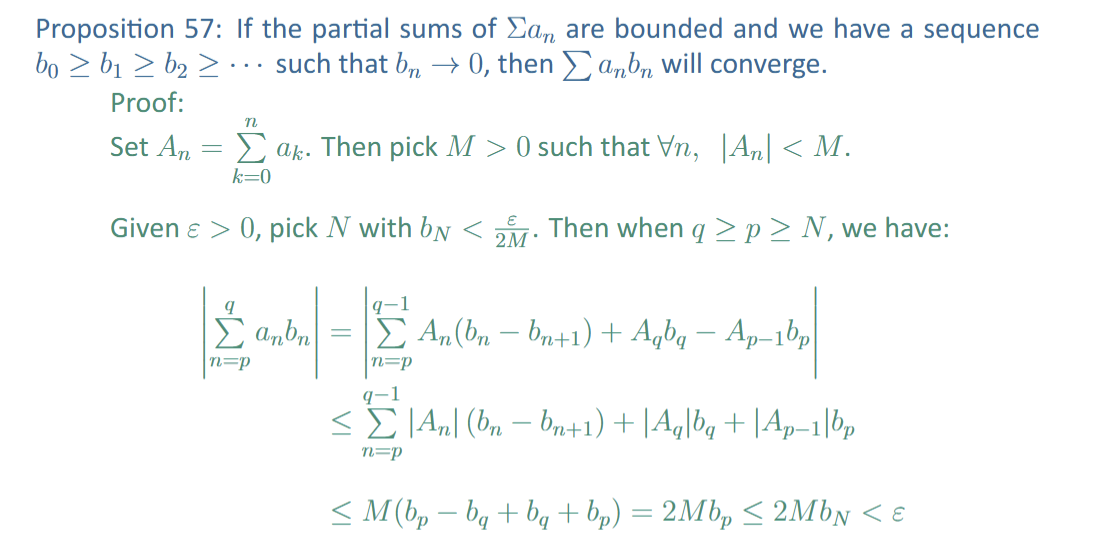
\includegraphics[scale=1]{Proof_HW3_math220a.png}\newpage\par}
	\end{itemize}
\end{myIndent}

\Hstatement\blab{Exercise III.2.1:} Show that $f(z) = |z|^2$ is complex differentiable only at the origin.

\begin{myIndent}\HexOne
	Identify $\mathbb{C}$ with $\mathbb{R}$ and consider $f$ as the function $f(x, y) = (x^2 + y^2, 0)$ going from $\mathbb{R}^2$ to $\mathbb{R}^2$. Then $f \in C^\infty(\mathbb{R}^2)$ with a derivative matrix $\left(\begin{smallmatrix}
	2x & 2y \\ 0 & 0
	\end{smallmatrix}\right)$. Now for $f$ to satisfy the Cauchy-Riemann equations (see the theorem on \inLinkRap{Cauchy-Riemann equations theorem}{page 296}) at a point $(x, y)$, we must have that $2x = 0$ and $-2y = 0$. Hence the only point where $f$ is complex differentiable is at\\ $(0, 0) = 0 + i0$.\retTwo
\end{myIndent}

\Hstatement\blab{Exercise III.2.3:} Show that $\lim_{n \to \infty} n^{1/n} = 1$.
\begin{myIndent}\HexOne
	If you want to prove this theorem without using logarithms (because you hadn't defined logarithms yet when you first relied on this fact), then here is the proof from math 140a:

	{\centering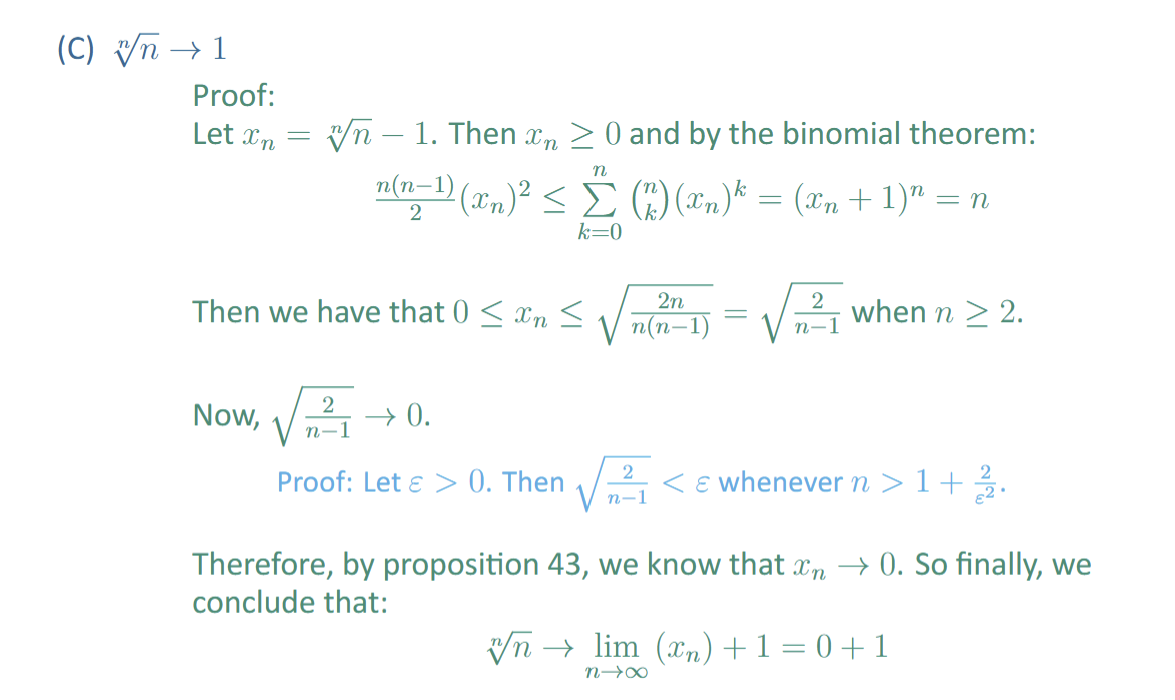
\includegraphics[scale=1]{Proof2_HW3_math220a.png}\retTwo\par}

	If you are willing to rely on logarithms and calculus though, then here is a slicker proof:
	\begin{myIndent}\HexTwoP
		Note that $\log(n^{1/n}) = \frac{1}{n}\log(n)$ for all $n$. Then by L'Hôpital's rule we have that $\lim_{x \to \infty}x^{-1}\log(x) = \lim_{x \to \infty}(1)^{-1}\frac{1}{x} = 0$. And hence $\log(n^{1/n}) \to 0$ as $n \to \infty$.\retTwo

		Finally, since $\exp$ is continuous, we have that $n^{1/n} = \exp(\log(n^{1/n})) \to \exp(0) = 1$ as $n \to \infty$.\retTwo
	\end{myIndent}
\end{myIndent}

\blab{Exercise III.2.19:} Let $G$ be a region and define $G^* = \{z : \overline{z} \in G\}$. If $f: G \to \mathbb{C}$ is holomorphic prove that $f^* : G^* \to \mathbb{C}$ defined by $f^*(z) = \overline{f(\overline{z})}$ is also holomorphic.

\begin{myIndent}\HexOne
	Once again identify $\mathbb{C}$ with $\mathbb{R}^2$ and write $f$ as $f(x, y) = (u(x, y), v(x, y))$. Then we have that $f^*(x, y) = (u(x, -y), -v(x, -y))$. And since $f$ is $C^1$, we can calculate that the derivative matrix of $f^*$ is $\Df (f^*) = \left(\begin{smallmatrix}
	u_x(x, -y) & -u_y(x, -y) \\ -v_x(x, -y) & v_y(x, y)
	\end{smallmatrix}\right)$.\retTwo

	Firstly, this shows that $f^*$ is also $C^1$ since all the partial derivatives of $f^*$ are continuous. Also, this shows that if $f$ satisfies the Cauchy-Riemann ewquations, then so does $f^*$. Hence $f$ being holomorphic on $G$ implies $f^*$ is as well.\retTwo
\end{myIndent}

\mySepTwo\retTwo





% ~~~~~~~~~~~~~~~~~~~~~~~~~~~~~~~~~~~~~~~~~~~~~~

\hypertarget{Ergodic reading group notes 3}{}

\hypertarget{existence and uniqueness diff eq notes}{}

\hypertarget{page 251 reference}{}
\hypertarget{page 271 reference}{}
\hypertarget{page 270 reference}{}
\hypertarget{Alireza theorem page 271}{}
\hypertarget{Cauchy's theorem page 271}{}

\hypertarget{math 241a lecture 5}{}
\hypertarget{math 200a lecture 9}{}
\hypertarget{math 220a lecture 9}{}


\hypertarget{page 284 reference example 1.2.1}{}

\hypertarget{idk reference 2}{}

\hypertarget{math 220a theorem II.2.3}{}
\hypertarget{Cauchy-Riemann equations theorem}{}



\end{document}



% \hTwo Suppose $|G| = pq$ where $p < q$ are prime numbers. Then $s_q = 1$. Hence there exists a unique Sylow $q$-subgroup $Q$. Furthermore, $Q \lhd G$ and $Q$ is cylic with order $q$.\retTwo

% Next, let $P$ by a Sylow $p$-subgroup. Then because $Q \lhd G$, we have that $PQ < G$. Also, $|P \cap Q| \divides \gcd(p, q) = 1$. So, $P \cap Q = \{1\}$ and from there it follows that $|PQ| = pq = |G|$. So $G / Q = PQ / Q \cong P / (P \cap Q) \cong P$.

